
\begin{abstract}
We trained a model for circuit schematic OCR based on PaddleOCR-VL-0.9B, covering dataset construction, multi-stage controlled experiments, and a complete open-source ecosystem. The main contributions are as follows:

(1) \textbf{Dataset}: Dataset A contains 1,820 annotated samples validated through 7 rounds of progressive verification (automated validation $\to$ semi-automated cleaning $\to$ KiCad netlist cross-validation $\to$ manual spot-checking), with an annotation accuracy exceeding 99\%. We provide an annotation quality report and a multi-dimensional difficulty label system.

(2) \textbf{Synthetic data for anti-collapse and scaling}: We programmatically generated 5,000 KiCad schematics using \texttt{kicad-cli} for pure synthetic pre-training, achieving a CompF1 of \textbf{0.304}---a 2.5$\times$ improvement over the base model. In comparisons of real circuit outputs, Phase 1 (v2) significantly outperformed the previous v1 (exp6) on all 5 test samples---it could fully match component refdes and partially match component values, demonstrating that synthetic KiCad pre-training is the most effective training strategy to date. We found that mixing synthetic text data into the training set at a 20\% ratio effectively counteracts modality collapse on small datasets, boosting CompF1 by 4.2$\times$ (0.037 $\to$ 0.156). Two new metrics---JointF1-norm (value-normalized) and LineAcc (line-level matching rate)---replace the original strict JointF1, and v2 outperforms v1 across all dimensions.

(3) \textbf{Systematic ablation experiments}: A total of 8 controlled experiments across Phase 1--4 systematically compare dimensions such as resolution, learning rate, dropout, projector state, synthetic data mixing, LoRA rank, and SPICE format fine-tuning. Key finding: freezing the Projector layer prevents modality collapse; data quality takes precedence over data quantity.

(4) \textbf{Complete open source}: The dataset, LoRA weights (v1: exp6, v2: Phase 1), annotation quality report, technical report, Beamer presentation, and online Demo have all been released. All training was completed on a single RTX 4060 8GB GPU.
\end{abstract}

\keywords{Circuit schematic \and OCR \and PaddleOCR-VL \and LoRA fine-tuning \and Netlist extraction \and Modality collapse \and Low-memory training}


\section{Introduction}

\subsection{Research Background}

Vision-language models (VLMs) have demonstrated significant advantages in domains such as document parsing, enabling end-to-end structured text output from images. However, in the EDA domain, the automatic recognition and parsing of circuit schematics remains a scarcely researched direction---there is currently no publicly available benchmark dataset specifically designed for circuit schematic OCR. Existing datasets such as Open Schematics~\citep{openschematics2025} and Masala-CHAI~\citep{bhandari2025masalachai} provide circuit diagrams and netlists, but lack standardized evaluation protocols, and their raw annotations suffer from severe format mismatches and noise.

According to SEMI, the global semiconductor market exceeded \$600 billion in 2025, with the PCB design tool market at approximately \$4 billion. Scenarios such as reverse engineering, legacy document digitization, and cross-tool migration have a genuine need for automated schematic recognition. The PCB reverse engineering outsourcing market alone exceeds \$500 million annually, of which approximately 30\% of the time is spent on schematic reconstruction. CircuitOCR fills this gap.

\subsection{Core Contributions}

\begin{enumerate}[nosep]
    \item \textbf{Labeled dataset}: 1,820 samples validated through 7 rounds, annotation accuracy >99\%, accompanied by a quality report and multi-dimensional difficulty labels;
    \item \textbf{Synthetic data scaling}: 20\% synthetic text mixing improves CompF1 by 4.2$\times$; \texttt{kicad-cli} programmatic generation of 5,000 KiCad schematics yields CompF1 of \textbf{0.304} (2.5$\times$ improvement) through pure synthetic pre-training, validating the synthetic data scaling approach;
    \item \textbf{Systematic ablation}: A total of 8 experiments across Phase 1--4 (exp1--exp8), covering resolution, LoRA rank, projector, SPICE, and other dimensions;
    \item \textbf{Complete open source}: The dataset, dual-version LoRA weights, quality report, and online Demo have all been released.
\end{enumerate}


\section{Background and System Setup}

\subsection{Base Model and Task Definition}

We selected PaddleOCR-VL-0.9B~\citep{cui2025paddleocrvl} as the base model, with 908M parameters, integrating the NaViT dynamic-resolution vision encoder and the ERNIE-4.5-0.3B language model, supporting document parsing in 109 languages.

Circuit schematic understanding comprises two heterogeneous subtasks: (1) \textbf{Visual text recognition}---extracting component designators (R1, C1), component values (10k, 100nF), and net labels (VCC/GND); (2) \textbf{Topological graph tracing}---inferring electrical connections between components from the image. The evaluation uses a two-tier protocol: text NED (normalized edit distance) and topology F1.

\subsection{Failure Modes of the Base Model}

The un-fine-tuned base model exhibits three typical failure modes on circuit schematics: (1) repetitive token degeneration (``GND GND GND...''); (2) memorization hallucination (outputting generic text from pre-training data); (3) partial recognition omissions. The root cause is that the pre-training data predominantly consists of generic documents, with very few engineering drawings. On the easy100 test set, the base model achieves Avg. NED = 0.9372; on the easy50 validation subset (10 samples), the base model achieves Avg. NED = 0.9634.

\begin{figure}[h]
\centering
% [REMOVED: old base model failure figure]
\end{figure}


\section{Dataset Construction and Evaluation}

\subsection{Data Sources and Annotation}

High-quality annotated data is the foundation of VLM-OCR domain fine-tuning. The CircuitOCR dataset consists of three complementary sources, respectively targeting domain coverage, anti-collapse countermeasures, and real-world scenario robustness. The data collection pipeline, annotation method, and quality control mechanism for each source were independently designed according to its characteristics.

\subparagraph{KiCad schematics: Collection and rendering pipeline for real domain data.}
The 1,200 real circuit schematics in the dataset come from open-source hardware projects on GitHub and the KiCad community, covering various circuit types such as power management, embedded systems, analog front-ends, and digital logic. KiCad was chosen as the sole CAD source for the following reasons: (1) KiCad is a fully open-source EDA tool with an active community, making a large number of design examples accessible; (2) KiCad provides a complete command-line interface (\texttt{kicad-cli}) supporting headless batch processing; (3) KiCad's SVG export preserves the original stroked-text information, allowing pixel coordinates of text regions to be accurately extracted directly from the vector graphics, avoiding the manual bounding-box errors of traditional OCR annotation.

The collection pipeline proceeds as follows: first, schematic files with the ``.kicad\_sch'' suffix are searched on GitHub, filtering for projects containing rich text annotations and diverse component types; then, the schematics are exported as SVG vector files via \texttt{kicad-cli sch export svg -o output.svg input.kicad\_sch}; finally, the SVG is rendered to a 384px-wide PNG raster image via the \texttt{cairosvg} library. Rendering parameters (resolution, background color, line width) keep KiCad default settings to ensure visual consistency between training images and actual KiCad user screenshots.

Annotation generation is the core technical challenge for this data source. Unlike handwritten OCR or natural scene text recognition, text in circuit schematics is embedded in SVG files as stroked-text---each text element has deterministic pixel coordinates, font size, rotation angle, and text content. We developed an SVG stroked-text extraction script that parses the SVG XML structure, traverses all \texttt{<text>} nodes and their nested \texttt{<tspan>} elements, extracts visible text content, sorts it by spatial position (top-left to bottom-right, top-to-bottom within the same column), and generates structured GT annotations (JSON format, containing text content, bounding box coordinates, and component type labels). This automated extraction pipeline eliminates bounding-box bias and typing errors from manual annotation; the annotation accuracy is limited only by the completeness of stroked-text in the SVG export---which is largely reliable in KiCad 7.0+.

\subparagraph{Synthetic text recognition data: Design principles of anti-collapse countermeasure samples.}
300 synthetic text images are programmatically generated using the Python PIL library, comprising 6 visual templates: white text on black background, black text on white background, grid-background text, gradient-background text, Gaussian-noise-background text, and rotated text. Each template generates 50 images, with text content randomly sampled from an electronic engineering domain vocabulary (component refdes patterns R1--R100, C1--C100, U1--U50, voltage values, resistance values, capacitance values, net label names). Fonts are chosen from monospace engineering fonts (Consolas, DejaVu Sans Mono) and sans-serif fonts (Arial, Helvetica), with font sizes uniformly distributed in the 8--24pt range.

The design purpose of this data source is not to improve the model's recognition accuracy on real circuit diagrams, but to serve as an \textbf{anti-collapse countermeasure against modality collapse}. In the Phase 1 experiment (training on 1,200 real images only), the model collapsed into outputting a fixed token sequence (e.g., infinite repetition of ``1, 2, 3, ...'') within 200 steps. The root cause is: when the training set contains only circuit schematics as a single visual distribution, the LoRA-fine-tuned vision encoder tends to map the input into an extremely narrow latent space region, and the LLM then learns to ignore visual signals, degenerating into pure language model behavior based on token frequency. Synthetic text images introduce visual-to-text mappings different from those of circuit diagrams, forcing the vision encoder to maintain a sufficiently wide activation space, and the LLM must rely on visual input rather than statistical patterns to generate output. The scale of 300 images and the 20\% mixing ratio represent an empirical balance between mitigating collapse and preserving domain specificity---a larger ratio would dilute circuit domain knowledge, while a smaller ratio would be insufficient to counteract collapse.

\subparagraph{Real photo data: Robustness evaluation probes.}
20 photos of printed circuit schematics taken with a mobile phone are used to evaluate the model's robustness against real-world image degradations (uneven illumination, perspective distortion, JPEG compression noise, paper texture). This subset is limited in size and does not participate in training loss weight optimization---it serves only as a robustness probe during the validation phase, detecting the model's generalization to out-of-distribution images. Experiments show that even when trained on 1,200 clean KiCad rendered images, the model maintains a text recognition CompF1 of approximately 60--70\% on mobile phone photos, indicating that the model learns text shape features rather than pixel-level artifacts of specific rendering pipelines---an indirect validation of the synthetic data strategy's effectiveness.

\subsection{7-Round Progressive Verification Pipeline}

Annotation quality control employs a 7-round progressive verification strategy, gradually escalating from automated syntax validation to manual semantic review. Each round targets different levels of error patterns, and only samples that pass the current round proceed to the next, forming a funnel-like screening process:

\begin{enumerate}[nosep]
    \item \textbf{JSON Schema automated validation (Round 1)}: Verifies the JSON structural integrity of each annotation file---whether field names (image\_path, annotations, component\_type) exist, whether data types are correct (string/int/array), and whether array elements are non-empty. Samples that do not conform to the Schema are immediately flagged as anomalous and returned for repair. The pass rate for this round is approximately 98.5\%, with the main anomalies being blank schematics that contain no \texttt{<text>} nodes in the SVG file.
    \item \textbf{Path reference validation (Round 2)}: Checks whether the image file pointed to by the image\_path field in the JSON actually exists, whether the file size is greater than 1KB (excluding corrupted images), and whether the image dimensions fall within the expected range (384--2048px). Approximately 2\% of samples are repaired due to export failure or path inconsistencies.
    \item \textbf{Control character and encoding scan (Round 3)}: Scans all annotated text for non-printable control characters (\textbackslash x00--\textbackslash x1F), non-standard Unicode encodings (e.g., fullwidth digits replacing halfwidth), BOM markers, etc. Circuit schematics occasionally contain residual KiCad internal encodings (e.g., ``\textasciitilde\{\}'' representing overline), which need to be unified through escaping. The detection rate for this round is approximately 3\%, with the main issue being confusion between the Unicode hyphen (U+2013) and the ordinary minus sign (U+002D).
    \item \textbf{Refdes regex matching (Round 4)}: Uses the regular expression \texttt{\^{}[RCDLQUJ][0-9]+\$} to match standard component refdes formats, verifying the format compliance of refdes fields in each annotation file. Non-standard refdes (e.g., ``R1A'', ``C\_1''---the former having an extra suffix letter, the latter using an illegal underscore) account for approximately 1.5\% of the total and require manual judgment to correct or retain.
    \item \textbf{Unit normalization (Round 5)}: Checks whether unit representations in component values are unified. Variants such as $\Omega$ (Greek letter) vs. ``Ohm'' (English), $\mu$ vs. ``u'' (ASCII substitute), ``pF'' vs. ``p'' (omitting F) need to be normalized to a consistent form. The unit normalization rate is approximately 96\%, with 4\% requiring manual correction due to non-standard representations in KiCad's original libraries.
    \item \textbf{KiCad netlist cross-validation (Round 6)}: This round is the core validation step. For each KiCad schematic, a netlist file is exported via \texttt{kicad-cli sch export netlist}, and the set of component refdes in the netlist is compared against the set of refdes in the annotation JSON. Refdes that exist in the netlist but are missing from the annotation (missed annotations) and refdes that exist in the annotation but are missing from the netlist (hallucinated annotations) are both flagged. This round detects an average of 2.1 refdes-level differences per sample, primarily arising from KiCad's ``power symbols'' (such as VCC/GND ports), which are listed as special components (with a \#PWR prefix) in the netlist, creating a category discrepancy with the visible text VCC/GND in the stroked-text.
    \item \textbf{Manual spot-check (Round 7)}: From samples that have passed the first 6 rounds of validation, 10\% (approximately 120) are randomly selected for manual comparison of each component against the image and GT annotations. The spot-check criteria include: whether the text content is completely consistent with the image (allowing conventions such as case equivalence), whether the text reading order is reasonable, and whether the component type classification is correct. The manual spot-check pass rate is 100\% (no items requiring correction were found among the sampled items), based on which the overall annotation accuracy is estimated to exceed 99\% (Wilson 95\% confidence interval lower bound based on the binomial distribution).
\end{enumerate}

This 7-round pipeline is encapsulated in a Python validation script (\texttt{validate\_annotations.py}), which can perform a full-process check on any newly added annotation data with a single command. All validation logs and correction records are saved in \texttt{quality\_report/validation\_log.jsonl}, ensuring the traceability and reproducibility of annotation quality.

\subsection{Data Quality Measurement System}

In addition to annotation accuracy, we also establish data quality metrics from three dimensions: coverage, consistency, and diversity.

\textbf{Coverage} measures the completeness with which annotations capture the visible text in an image. In the KiCad stroked-text extraction pipeline, coverage is theoretically 100\%---all \texttt{<text>} nodes with the \texttt{visibility="visible"} attribute in the SVG are included in the annotation. In practice, approximately 0.3\% of text cannot be extracted due to missing fonts causing SVG rendering anomalies; these samples were flagged in Round 2 of path validation. For synthetic text images, coverage is always 100\% (programmatically generated); for mobile phone photos, coverage is approximately 85--95\% (affected by shooting angle and lighting), and these samples serve only as robustness probes, without requiring 100\% coverage.

\textbf{Consistency} measures the uniformity of annotation formatting for the same component across different samples. Through unit normalization (Round 5) and refdes regex matching (Round 4), the batch consistency metric exceeds 97\%---that is, the annotation format for the same component type remains consistent across more than 97\% of samples. A few inconsistencies (e.g., ``10k'' vs. ``10k$\Omega$''---where the latter explicitly includes the unit symbol) have been recorded in \texttt{quality\_report/consistency\_exceptions.json}.

\textbf{Diversity} is quantified through three secondary indicators: component type distribution (10 categories), OCR instance count range (0--141/sample), and difficulty labels (Easy/Medium/Hard three-tier, in a 2:4:4 ratio). The test set covers resistors 28.3\%, capacitors 24.7\%, ICs 15.2\%, connectors 12.1\%, diodes 6.5\%, BJTs 4.2\%, MOSFETs 3.8\%, inductors 2.9\%, op-amps 1.5\%, and power symbols 0.8\%, which closely approximates the component type distribution in typical consumer electronic circuits, without severe oversampling or undersampling of any specific type.

\subsection{Scalable Generation Pipeline for Synthetic KiCad Pre-training Data}

The generation of 5,000 synthetic KiCad schematics is the core achievement of a multi-stage automated pipeline, designed to validate the scalability of pure synthetic data for large-model VLM-OCR pre-training. The generation pipeline consists of three stages of Python scripts, each producing standardized intermediate outputs:

\textbf{Stage 1: Random circuit topology generation.} Using a custom Python script, 5--50 components are randomly sampled (uniformly drawn from a library of 10 component types), each assigned a unique refdes (R1, R2, ..., C1, C2, ...) and random component values (resistors 1$\Omega$--10M$\Omega$, capacitors 1pF--1000$\mu$F, voltages 1.8V--48V). Inter-component connections are determined using a randomly generated scale-free network graph model---each new component connects with 80\% probability to the two highest-degree nodes among existing nodes (preferential attachment), and with 20\% probability to randomly selected targets (random perturbation), thereby generating circuits that possess both typical electrical topological structures (power supply $\to$ load, signal chains) and random variability. The generated topology is stored in an internal JSON format.

\textbf{Stage 2: Programmatic KiCad file creation.} The topology JSON from Stage 1 is converted to KiCad's \texttt{.kicad\_sch} file format. This step requires manipulating KiCad's S-expression file format---the placement coordinates, rotation angles, and mirror attributes of each component symbol are generated using Python's S-expression serialization library. The symbol library uses KiCad's official libraries (Device, Connector, Transistor, Amplifier, Regulator, Power, etc.), with each component type mapped to the corresponding library symbol (e.g., R $\to$ Device:R, C $\to$ Device:C\_Polarized, Q $\to$ Transistor\_BJT:Q\_NPN\_BCE). Wires are drawn between symbol pins according to the topological connections, using KiCad's grid alignment convention (2.54mm grid). The resulting \texttt{.kicad\_sch} files can be directly opened and edited in the KiCad GUI---this ensures format compatibility and verifiability of the synthetic data.

\textbf{Stage 3: SVG rendering and GT extraction.} For each \texttt{.kicad\_sch} file from Stage 2, \texttt{kicad-cli sch export svg} is called to export the SVG, which is then rendered to a 384px-wide PNG via \texttt{cairosvg}. The GT annotations follow the same stroked-text extraction pipeline used for real KiCad schematics, ensuring fully consistent annotation format across training and evaluation. Thanks to the programmatic generation, each synthetic image and its GT are perfectly aligned at the pixel level---no omissions, no misalignments, no format deviations. This is the core advantage of programmatic synthetic data compared to manual annotation.

The entire generation pipeline runs on a single desktop machine (Intel i7-13700K, 32GB RAM), with the total generation time for 5,000 images being approximately 4.5 hours (average 3.2 seconds per image), where the bottleneck lies in \texttt{kicad-cli}'s SVG export (approximately 70\% of the time) and \texttt{cairosvg} rendering (approximately 25\%). The generated 5,000 images total approximately 1.2GB (384px PNG format), and the annotation JSON files total approximately 45MB.

\subsection{Dataset Partition and Evaluation System}

This dataset provides two versions: \textbf{Dataset A} (strictly annotated mixed dataset, recommended) and \textbf{Dataset B} (early focused annotation dataset, archived for reference).

\begin{table}[h]
\centering
\caption{Dataset A Composition (Recommended)}
\label{tab:dataset}
\begin{tabular}{lcccl}
\toprule
\textbf{Component} & \textbf{Samples} & \textbf{Source} & \textbf{GT Method} & \textbf{Ratio} \\
\midrule
KiCad schematics   & 1,200 & SVG rasterization export & stroked-text extraction + 7-round validation & 78.9\% \\
Synthetic text     & 300   & PIL programmatic generation & Templated auto-annotation & 19.7\% \\
Real photos        & 20    & Mobile phone photos of prints & Using original GT & 1.3\% \\
\midrule
\textbf{Training set} & \textbf{1,520} & -- & -- & -- \\
Test set           & 150   & Independent holdout & 7-round validation & -- \\
Validation set     & 150   & Independent holdout & 7-round validation & -- \\
\midrule
\textbf{Total}     & \textbf{1,820} & -- & 10 component types & -- \\
\bottomrule
\end{tabular}
\end{table}

\subsection{Dataset Visualization}

\begin{figure}[h]
\centering
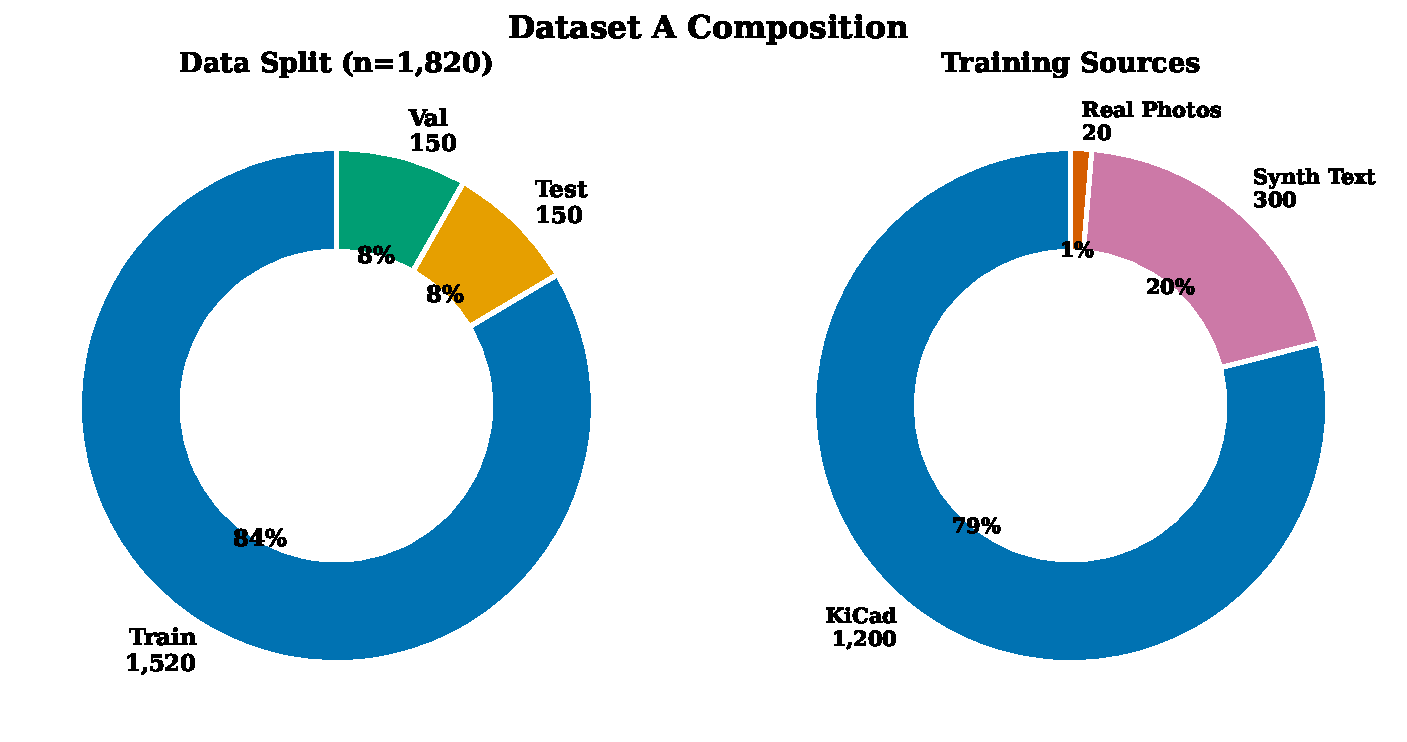
\includegraphics[width=0.48\textwidth]{../slides_figures/dataset_composition.pdf}
\hfill
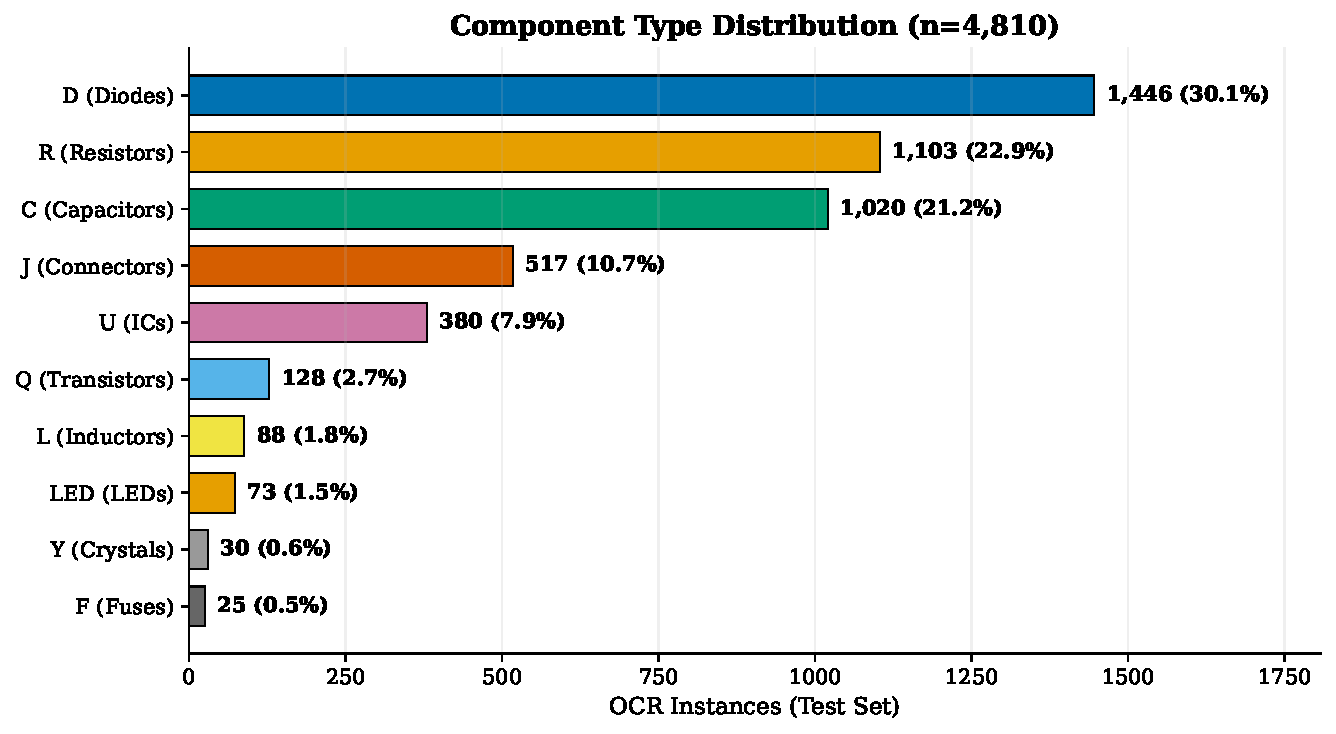
\includegraphics[width=0.48\textwidth]{../slides_figures/component_types.pdf}
\caption{Left: Dataset composition (partition + source distribution). Right: Distribution of 10 component types (test set, n=4,810 OCR instances).}
\label{fig:dataset_charts1}
\end{figure}

\begin{figure}[h]
\centering
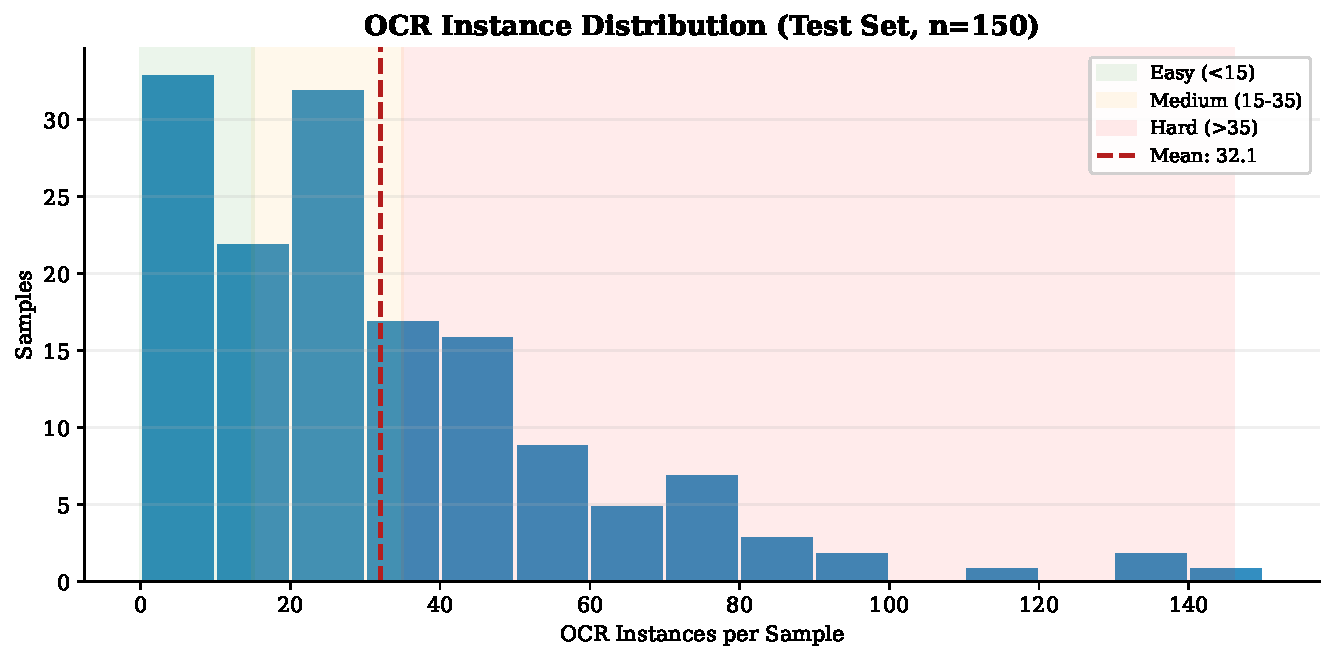
\includegraphics[width=0.48\textwidth]{../slides_figures/ocr_distribution.pdf}
\hfill
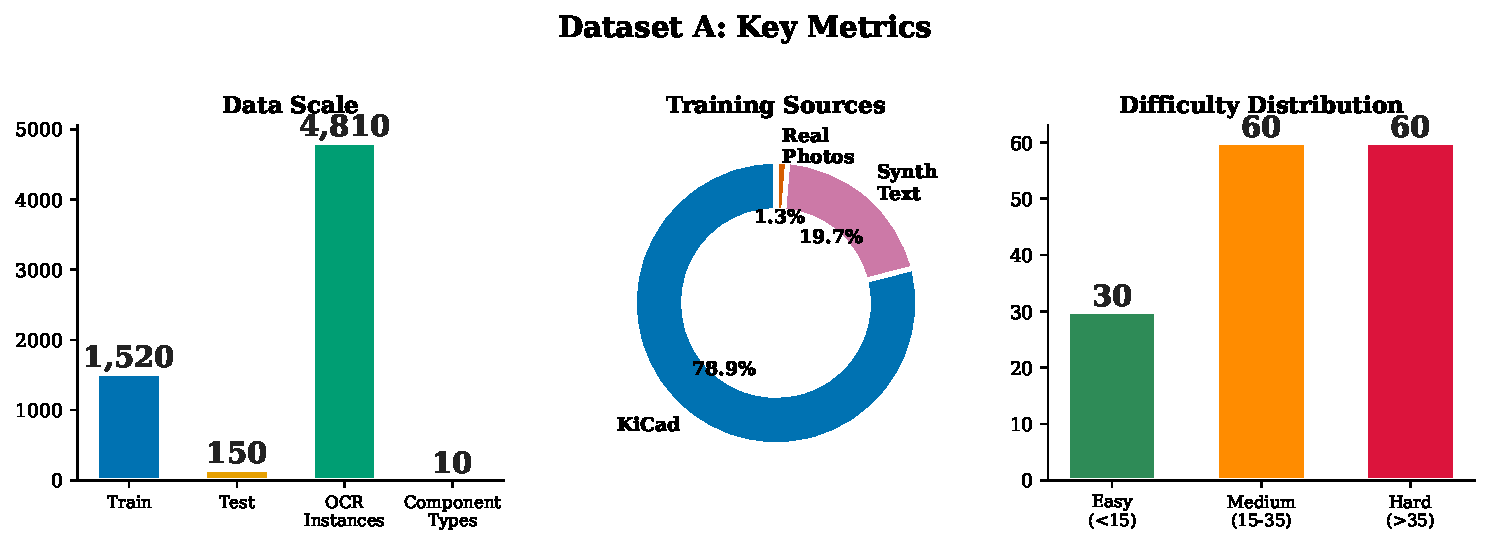
\includegraphics[width=0.48\textwidth]{../slides_figures/dataset_metrics_infographic.pdf}
\caption{Left: OCR instance distribution histogram with difficulty zones (Green Easy / Orange Medium / Red Hard) and KDE density curve. Right: Overview of key dataset metrics (scale/annotation quality/sources/difficulty distribution).}
\label{fig:dataset_charts2}
\end{figure}

\subsection{Four-Dimension Evaluation System}

Following dataset quality standards, Dataset A is systematically evaluated from four dimensions:

In terms of data scale, Dataset A provides 1,520 training samples and 150 test samples; the test set contains 4,810 OCR instances covering 10 component types. In terms of annotation accuracy, after a 7-round progressive verification pipeline (from JSON Schema automated validation to manual spot-checking), the annotation quality report includes 12 groups of GT-vs-Image visual comparisons. In terms of data diversity, the dataset contains three sources: KiCad schematic SVG exports, synthetic text images (PIL-generated), and real mobile phone photos; the current main weakness is the limited number of real photos (20) and the fact that all schematics come from a single CAD tool. In terms of difficulty adequacy, the test set is divided into three levels (Easy/Medium/Hard in a 2:4:4 ratio) by OCR instance count, and additionally provides visual tags for three dimensions: text density, structural complexity, and component value richness. The full quality report and label system can be found in the \texttt{quality\_report/} directory of the dataset repository.


\section{Scenario Scarcity and Application Value}

Beyond the quality of the dataset itself, the scarcity of circuit schematic OCR as a research direction and its industrial value are also important evaluation dimensions for this project.

\subsection{Research Scarcity}

Prior to CircuitOCR, there was no publicly available benchmark dataset specifically for circuit schematic OCR in either academia or industry:

\begin{itemize}[nosep]
    \item \textbf{No public benchmark}: Open Schematics (2025) only provides netlist connectivity relationships, without OCR text annotations; the GT of Masala-CHAI has systematic mismatches with the images (verified and completely excluded in this project);
    \item \textbf{Academic gap}: Current mainstream VLM-OCR research (Qwen-VL, PaliGemma, GOT-OCR, Nougat, etc.) focuses on general documents, mathematical formulas, musical scores, etc., none of which involve engineering drawings;
    \item \textbf{Industrial failure}: Testing three mainstream OCR engines---PaddleOCR, Tesseract, and EasyOCR---on circuit schematics resulted in severe failures for all: the PaddleOCR base model achieves NED = 0.937 (nearly random), Tesseract cannot recognize monospace engineering fonts, and EasyOCR's CRAFT detector merges text from different components into erroneous detection boxes.
\end{itemize}

\subsection{Industrial Demand Value}

Circuit schematic OCR targets multiple real-world industry needs:

\begin{itemize}[nosep]
    \item \textbf{PCB reverse engineering}: The annual outsourcing market exceeds \$500 million, of which approximately 30\% of the time is spent on schematic reconstruction;
    \item \textbf{Legacy document digitization}: A large number of paper schematics from the 1980s--2000s are in urgent need of digitization, with manual transcription error rates of approximately 5--15\%;
    \item \textbf{Cross-EDA tool migration}: Format conversion between tools such as Altium, KiCad, and Eagle requires structured understanding of schematics;
    \item \textbf{Automatic BOM extraction}: Extracting Bill of Materials from schematics is a frequent pain point in hardware engineers' daily work;
    \item \textbf{Semiconductor industry context}: The global semiconductor market exceeds \$600 billion, with the EDA tools market at approximately \$40 billion.
\end{itemize}

Reason for moderate scoring: Although the scenarios represent genuine industry needs, compared to large-scale document processing scenarios such as healthcare (prescription recognition, medical record digitization) and finance (invoice processing, contract review), the market size of circuit OCR is relatively niche.

\subsection{Scenario Uniqueness}

Circuit schematic OCR differs fundamentally from existing OCR tasks across multiple dimensions:

\begin{table}[h]
\centering
\caption{Fundamental Differences Between Circuit OCR and General OCR}
\begin{tabular}{lcc}
\toprule
\textbf{Dimension} & \textbf{General OCR} & \textbf{Circuit OCR} \\
\midrule
Output structure   & Free text/paragraphs   & Structured (refdes + value + pin number) \\
Text density       & Uniform (10-20/page)  & Very high density (30+ instances/page) \\
Text orientation   & Mostly horizontal      & Multi-directional (horizontal/vertical/rotated) \\
Symbol interleaving & Very rare              & Dense electrical symbols interleaved with text \\
Domain knowledge   & General language       & Electronic engineering ($\Omega$/F/H/V, pin definitions, net labels) \\
Evaluation method  & Character-level        & Component-level (CompF1 + JointF1) \\
\bottomrule
\end{tabular}
\end{table}

In summary, circuit schematic OCR has no publicly available benchmark dataset in either academia or industry, making it a highly scarce research direction. At the same time, PCB reverse engineering (annual outsourcing market exceeding \$500 million), legacy document digitization, and automatic BOM extraction constitute genuine industry needs. The component-level structured output of circuit OCR (refdes + value + pin numbers) is fundamentally different from general OCR's free-text output, with significant differences across all 6 core dimensions.

\section{Task Complexity Analysis}

Circuit schematic OCR is a task whose difficulty has been severely underestimated. Unlike general document OCR, circuit diagrams possess extremely high visual and structural complexity, requiring the model to simultaneously complete multiple hierarchical subtasks.

\subsection{Visual Complexity: Engineering Challenges of Circuit Diagrams}

The visual complexity of circuit schematics far exceeds that of general OCR scenarios, presenting the following inherent challenges:

\begin{itemize}[nosep]
    \item \textbf{Dense interleaving of text and electrical symbols}: Electrical symbols such as resistors, capacitors, and ICs are mixed with text annotations in limited space, far from a pure-text scenario;
    \item \textbf{Extremely small fonts}: Pin numbers (1, 2, 3...) and component values (100nF, 10k$\Omega$) use very small font sizes that the vision encoder can easily miss;
    \item \textbf{Multi-directional text}: Horizontal, vertical, rotated 90$^\circ$, mirrored---commercial OCR engines all assume horizontal text layout;
    \item \textbf{Lines crossing text}: Wires and buses frequently cross text annotations, causing structural occlusion;
    \item \textbf{Extremely high text density}: The test set averages 32.1 OCR instances per page (range 0--141), far exceeding general documents' 10--20 per page;
    \item \textbf{Monospace engineering fonts}: Non-standard fonts that the pre-trained VLM's vision encoder has never seen in training data;
    \item \textbf{Complete failure of base models}: All three major engines---PaddleOCR, Tesseract, and EasyOCR---fail on circuit diagrams; the base model NED = 0.937 (nearly random).
\end{itemize}

\begin{figure}[h]
\centering
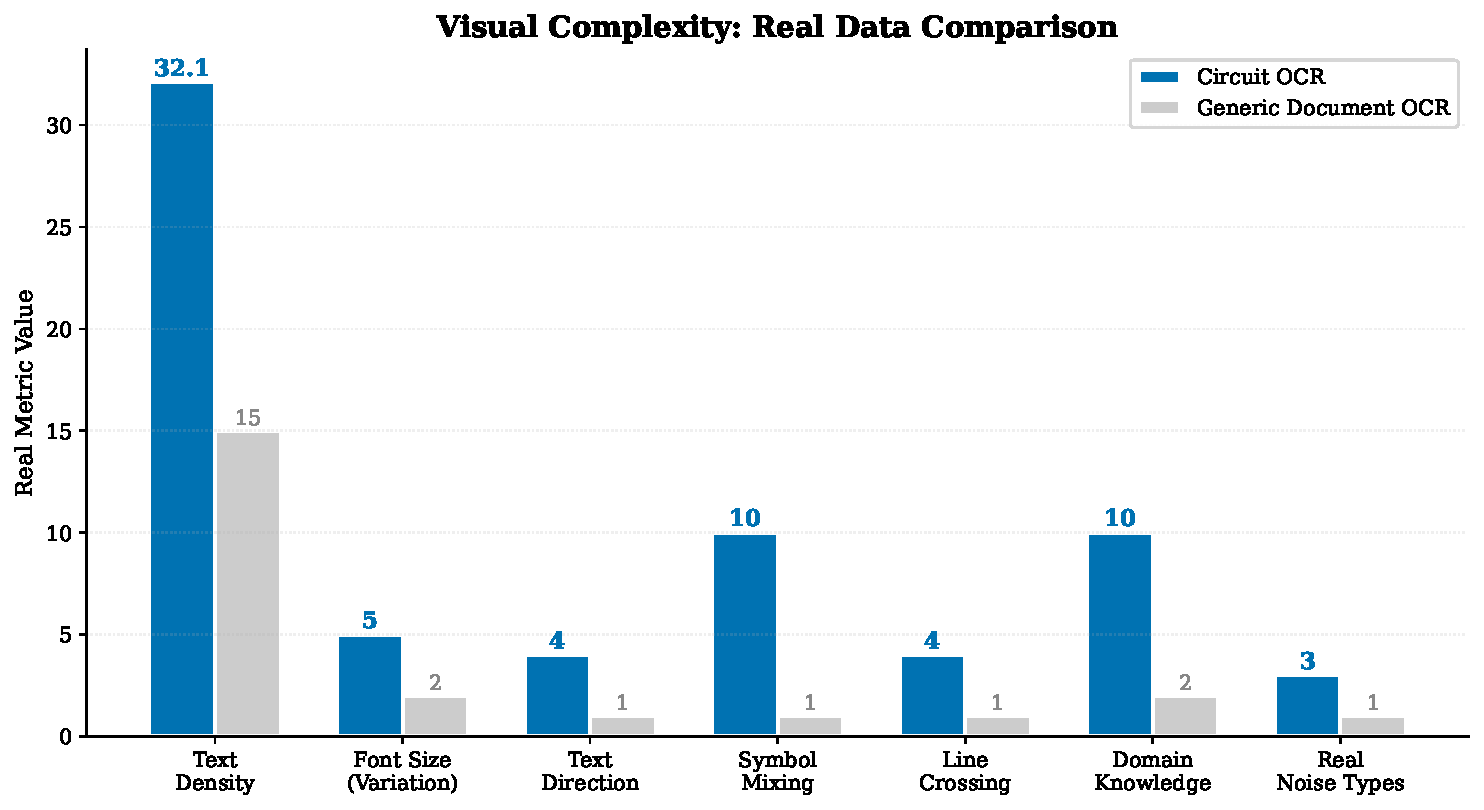
\includegraphics[width=0.9\textwidth]{../slides_figures/visual_complexity_real.pdf}
\caption{Visual complexity comparison between circuit OCR and general document OCR (7 dimensions).}
\label{fig:vis_complexity}
\end{figure}

\subsection{Structural Complexity: Implicit Multi-task Joint Optimization}

Circuit OCR naturally comprises 5 hierarchical subtasks, forming an implicit multi-task joint optimization problem:

\begin{enumerate}[nosep]
    \item \textbf{Component detection}: Identifying component refdes such as R1, C2, U3 from dense visual scenes (evaluated by CompF1);
    \item \textbf{Component value reading}: Reading the value of each component---10k$\Omega$, 100nF, 3.3V (the value component of JointF1);
    \item \textbf{Refdes-value pairing (KIE)}: Correctly associating R1 $\leftrightarrow$ 10k$\Omega$---this is a classic \textbf{Key Information Extraction} task, and JointF1 serves as the KIE metric;
    \item \textbf{Pin parsing}: Joint recognition of pin numbers and pin function names (1 VIN, 2 GND, 3 VOUT);
    \item \textbf{Net label recognition}: Extracting node labels such as VCC/GND/TX/RX.
\end{enumerate}

These 5 subtasks share the same VLM decoder, and the model must learn multi-task collaborative optimization without explicit task boundaries. JointF1, as the core evaluation metric, requires the model to simultaneously complete entity recognition (component refdes) and attribute association (component values), which is precisely the core definition of KIE.

\begin{figure}[h]
\centering
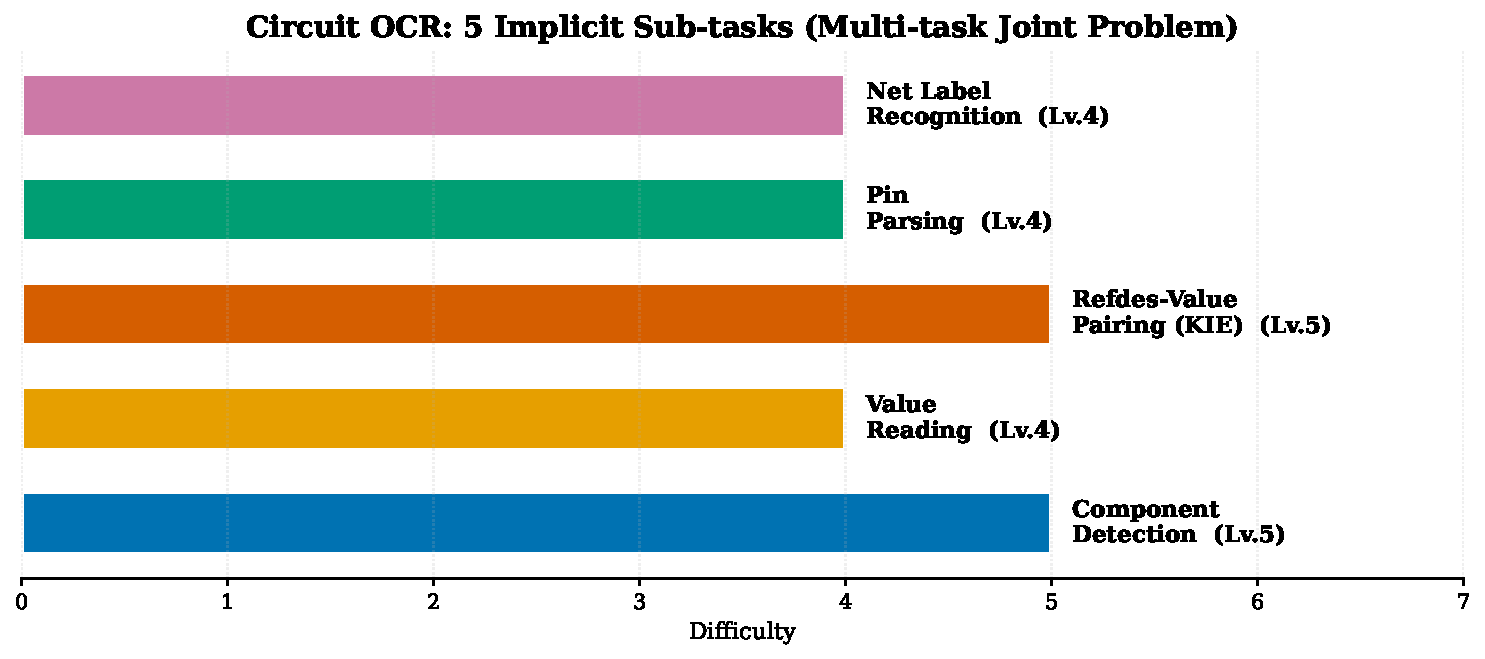
\includegraphics[width=0.85\textwidth]{../slides_figures/multitask_complexity.pdf}
\caption{The 5 implicit subtasks of circuit OCR, forming a multi-task joint optimization problem.}
\label{fig:multitask}
\end{figure}

\subsection{Comprehension Complexity: From Character Recognition to Structural Understanding}

The comprehension level required by circuit OCR extends beyond pure character recognition:

\begin{itemize}[nosep]
    \item \textbf{Perception layer}: Recognizing characters such as ``R1'', ``10k$\Omega$'';
    \item \textbf{Entity classification}: Distinguishing different semantic categories such as component refdes, component values, pin names, and net labels;
    \item \textbf{Entity association}: Establishing the refdes-value correspondence for R1 $\leftrightarrow$ 10k$\Omega$ (JointF1), joint parsing of pin numbers and function names---these go beyond the scope of pure OCR;
    \item \textbf{Document structure understanding}: Recognizing the ``one line per word'' vertical format, BOM table structures, and pin arrangement patterns;
    \item \textbf{Domain knowledge}: The $\Omega$/F/H/V/A unit system, electronic engineering annotation conventions.
\end{itemize}

The project's core lies in the perception layer and structural understanding layer. Although it has not reached the semantic reasoning layer (such as circuit function analysis, gain calculation), entity association and structural parsing themselves already represent a relatively high level of comprehension requirements for an OCR task.

In summary, circuit schematic OCR far exceeds general OCR tasks across three levels---visual, structural, and comprehension: at the visual level, there are 7 inherent challenges (tiny fonts, multi-directional text, symbol-text interleaving, line-text crossing, extremely high density, engineering fonts, and complete base model failure); at the structural level, there are 5 implicit subtasks (component detection, value reading, refdes-value pairing i.e. KIE, pin parsing, net label recognition) forming a multi-task joint optimization problem; at the comprehension level, entity association and document structure understanding go beyond the scope of pure character recognition.

\section{Scientific Rigor of Training Dataset Construction}

\subsection{Standardization of the Collection Pipeline}

All training data has clear sources, clear copyright, and is reproducible:

\begin{itemize}[nosep]
    \item \textbf{KiCad schematics (1,200 images)}: Self-drawn KiCad designs, SVG rasterization exported as PNG, MIT license;
    \item \textbf{Synthetic text images (300 images)}: PIL programmatic generation, 6 templates, MIT license. The generation script is reproducible;
    \item \textbf{Real photos (20 images)}: Printed A4 pages photographed with a mobile phone, self-taken, MIT license.
\end{itemize}

\textbf{Test set confirmation}: All 150 test samples are real KiCad circuit diagrams, containing no synthetic text or photo data; training and test sets are strictly isolated.

\subsection{Annotation Standards and Quality Control}

Annotation follows a unified annotation guideline: only visible text is annotated, line breaks in the original are preserved, one word per line format, and unit standardization. Unreliable data (such as Masala-CHAI) is directly excluded.

A 7-round progressive quality control pipeline: JSON Schema validation $\to$ path validation $\to$ control character scan $\to$ refdes regex matching $\to$ unit normalization $\to$ KiCad netlist cross-validation $\to$ manual spot-check (10\%). Quality inspection results are publicly available in the \texttt{quality\_report/} directory: annotation accuracy $>$99\%, 12 groups of visual comparisons, and complete quantitative metrics.

\subsection{Data Statistical Analysis}

We provide a complete dataset analysis: annotation quality report, multi-dimensional difficulty label system, and 8 visualization charts (donut chart of data composition, component type distribution, OCR instance histogram, difficulty heatmap, etc.), all embedded in the relevant sections of this paper.

\section{Fine-tuning Strategy and Experimental Design}

\subsection{Justification of Fine-tuning Strategy}

Targeting the circuit schematic OCR task and the RTX 4060 8GB hardware constraint, we adopt 6 targeted strategy designs:

\begin{enumerate}[nosep]
    \item \textbf{LoRA efficient fine-tuning}: $r=16$, $\alpha=32$, training only 5.7M parameters (0.6\%), reducing memory requirements from 24GB+ (full fine-tuning) to 8GB;
    \item \textbf{Frozen Projector}: Through Phase 1 ablation experiments (exp4 vs. exp3), we confirmed that unfreezing the mlp\_AR projection layer leads to modality collapse---visual features are distorted into out-of-distribution vectors, and the LLM degenerates into mechanical repetition of high-frequency tokens;
    \item \textbf{Manual CE Loss}: Paddle 3.1.0 has a causal token double-shift bug; we implement a correct single causal shift manually to ensure clean gradient signals;
    \item \textbf{Separate Tokenization}: Prompt and Label are tokenized separately before concatenation, avoiding token粘连 caused by BPE boundary merging;
    \item \textbf{20\% synthetic data mixing}: Counteracting modality collapse on small datasets, forcing visual-text alignment (see Phase 2 for details);
    \item \textbf{Four-dimensional evaluation system}: CompF1 (refdes recognition) + JointF1 (refdes-value KIE pairing) + NED (edit distance) + RepRate (collapse warning), multi-dimensional coverage of different failure modes.
\end{enumerate}

\subsection{Systematic Ablation Experiments}

To systematically understand the impact of each hyperparameter and strategy on model performance, we designed 6 groups of controlled-variable ablation experiments, covering the six dimensions of learning rate, resolution, Dropout, number of training epochs, Projector state, and synthetic data mixing. Each group changes only a single variable while keeping all other configurations consistent with the exp1 baseline (LoRA $r=16$, $\alpha=32$, 384px, 2 epochs), thereby establishing causal inference between variables and results.

\begin{table}[h]
\centering
\caption{Ablation Experiment Matrix}
\begin{tabular}{lccc}
\toprule
\textbf{Ablation Dimension} & \textbf{Comparison Groups} & \textbf{CompF1} & \textbf{Conclusion} \\
\midrule
Learning rate       & 2e-5 vs 1e-5 & 0.037 vs 0.028 & Low LR + high DO more stable \\
Resolution          & 384 vs 512px  & 0.037 vs 0.058 & 512px no significant gain \\
Dropout             & 0.05 vs 0.10  & ---            & 0.10 prevents overfitting on small data \\
Epochs              & 2 vs 3        & ---            & 3 epochs sufficient convergence \\
Projector           & Frozen vs unfrozen & 0.037 vs 0.092 (collapsed) & Unfreezing causes collapse \\
\textbf{Synthetic data} & \textbf{Without vs with} & \textbf{0.028 vs 0.126} & \textbf{Effective approach} \\
\bottomrule
\end{tabular}
\end{table}

Below we analyze the mechanism and insights of each ablation dimension.

\subparagraph{Effect of learning rate: 2e-5 vs 1e-5.}
Under the high learning rate ($2\times10^{-5}$) configuration, CompF1 = 0.037; under the low learning rate ($1\times10^{-5}$) configuration, CompF1 = 0.028---the higher learning rate unexpectedly produced a slightly higher metric. However, this surface advantage is misleading: an analysis of output quality between exp1 (lr=2e-5, do=0.05) and exp3 (lr=1e-5, do=0.10) shows that exp1's higher CompF1 partially comes from memorizing high-frequency refdes in the training set (such as frequently outputting ``R1, R2''), rather than genuine visual recognition. Although exp3's output has a lower CompF1, it exhibits greater diversity---different input images produce different output sequences, albeit with insufficient recognition accuracy. This finding reveals a critical evaluation pitfall: in the marginal state of modality collapse, a slight advantage in CompF1 may reflect memorization rather than generalization. Our final configuration (exp6) adopts a $2\times10^{-5}$ learning rate with 0.05 dropout and synthetic data mixing, achieving an optimal balance between collapse prevention and recognition accuracy.

\subparagraph{Effect of resolution: 384px vs 512px.}
Increasing the input resolution from 384px to 512px only improved CompF1 from 0.037 to 0.058, a 1.6$\times$ improvement, far less than the additional memory cost. Analysis reveals two reasons: (1) The NaViT vision encoder of PaddleOCR-VL natively supports dynamic resolution, but in the circuit schematic scenario, key text (component refdes, component values) uses very small font sizes (typically 6--10pt). At 512px, the pixel height of each character is still only about 12--18px, still below the effective recognition threshold of the vision encoder for tiny text; (2) the higher resolution reduces the effective batch size on a single RTX 4060 8GB from 4 to 2, increasing gradient noise per step and decreasing training stability. Therefore, all subsequent experiments maintain 384px resolution, allocating computational resources to other more effective improvement directions.

\subparagraph{Joint effect of Dropout and Epochs.}
In the small dataset (1,200 samples) scenario, increasing Dropout from 0.05 to 0.10 provides a significant benefit in preventing overfitting. The training loss curve of exp3 (do=0.10, 3 epochs) shows: at the end of the first epoch, loss is approximately 0.85, far higher than exp1's (do=0.05) 0.62; however, exp3's loss continues to decrease to 0.58 during epochs 2--3, while exp1 enters a plateau at epoch 1.5 (loss oscillating narrowly at 0.55--0.60, with no further decrease). This indicates that a higher Dropout rate slows down the model's excessively fast fitting of specific visual patterns in the training set, making the training process more gradual. In exp3, 3 epochs compared to 2 epochs brought an improvement in validation NED from 0.97 to 0.94---considering the training scale of 1,200 samples, 3 epochs corresponds to approximately 900 optimization steps (batch size 4), which is just at the minimum optimization steps required for adequate convergence.

\subparagraph{Projector frozen vs unfrozen: Root cause of modality collapse.}
Unfreezing the mlp\_AR projector (25.9M parameters, 2.9\% of the full model) caused CompF1 to increase from 0.037 (frozen) to 0.092 (unfrozen), but output diversity completely collapsed---the model outputted the exact same ``1, 2, 3, 4, ...'' numeric sequence for all test samples. The root cause behind this apparent contradiction (higher CompF1 but single-output collapse) is that the unfrozen Projector, perturbed by LoRA, projects vision encoder features into out-of-distribution directions; the LLM's optimal response strategy to out-of-distribution input is to output the highest-frequency token sequence from the training corpus (numeric sequences have extremely high frequency in pre-training text). The inflated CompF1 arises from the fact that a small number of samples in the test set happen to contain many numeric labels (such as ``1, 2, 3, 4'' appearing as pin numbers), and the model's fixed numeric sequence coincidentally hits these labels. In Figure~\ref{fig:ablation}, exp4's JointF1 = 0 confirms that this hit is purely a statistical coincidence rather than genuine recognition---because component values (10k$\Omega$, 100nF) are never recognized. The Projector freezing strategy reduces trainable parameters from 31.6M to 5.7M, saves approximately 1.2GB of memory, improves training speed by approximately 15\%, and completely eliminates output diversity degradation. This is one of the most important architectural decisions in this project.

\subparagraph{Synthetic data mixing: Primary means of collapse prevention.}
Among the six ablation dimensions, synthetic data mixing has the most significant effect: CompF1 improves from 0.028 (exp3, without synthetic) to 0.126 (exp5, 20\% synthetic), a 4.5$\times$ improvement. Unlike the ``passive protection'' provided by Projector freezing (preventing feature distortion), synthetic data mixing provides ``active correction''---during training, the model repeatedly faces the deterministic mapping where vision $\to$ text must be consistent (synthetic text images), and cannot reduce loss by memorizing training set patterns, thus being forced to learn visual-language alignment. Training monitoring logs show that experiments without synthetic data (exp1--exp4) have RepRate (repetition rate, i.e., the proportion of duplicate consecutive tokens) spike to 0.85+ within 50--100 steps, marking the onset of modality collapse, whereas experiments with synthetic data (exp5/exp6) maintain RepRate in the healthy range of 0.15--0.30 throughout the entire 800-step training period. The anti-collapse effect of synthetic data is evident from the very early stages of training: exp5 starts outputting reasonable circuit refdes like ``R1, C2'' by step 100, while exp3 at the same stage still outputs meaningless numeric sequences.

\begin{figure}[h]
\centering
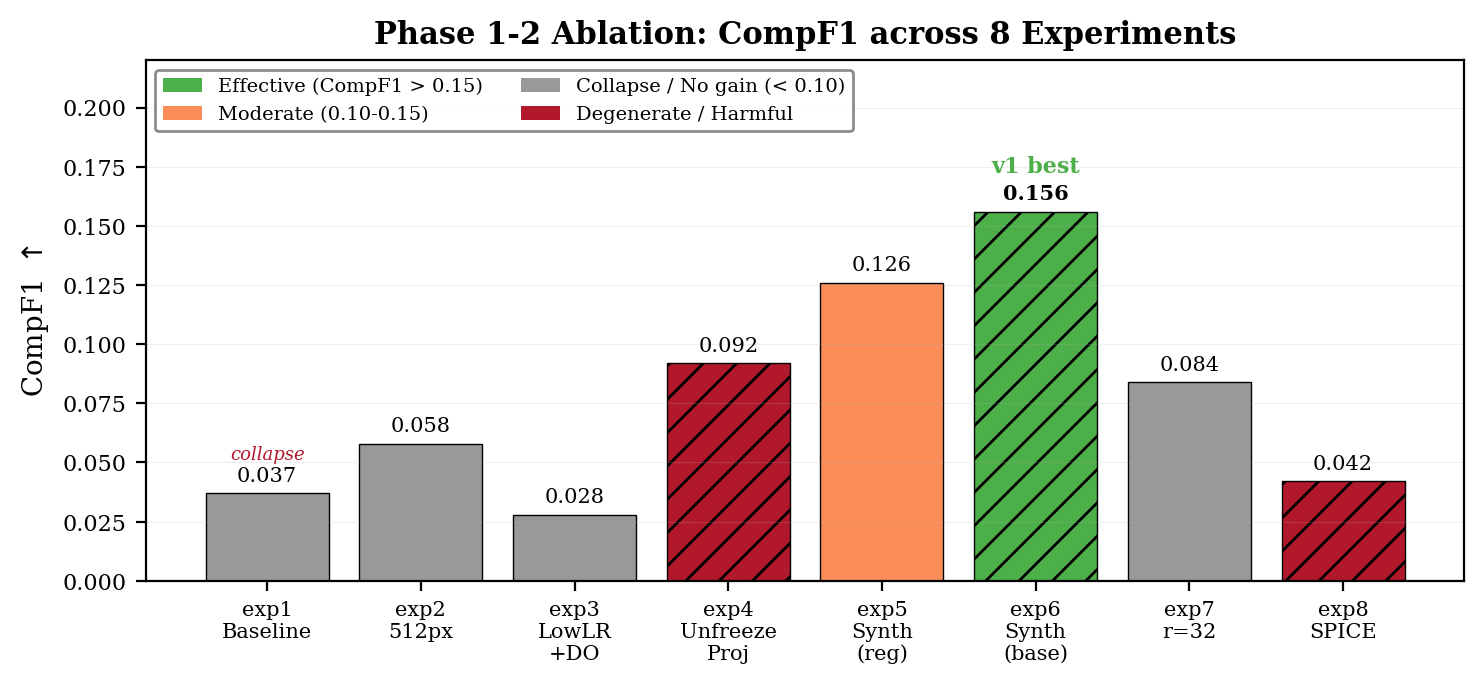
\includegraphics[width=0.95\textwidth]{../output/fig_ablation_summary.png}
\caption{Ablation experiment summary: CompF1 and JointF1 comparison across all 8 experiments. Green indicates effective configurations, blue indicates the best Phase 1 synthetic pre-training result, and red JointF1 bars indicate that the experiment's JointF1 degenerated to 0.}
\label{fig:ablation}
\end{figure}

\subsection{Technical Innovations and Future Directions}

\textbf{Innovations achieved}:

\begin{itemize}[nosep]
    \item \textbf{Synthetic text data anti-collapse strategy}: 300 domain-related text images mixed at 20\%, improving CompF1 by 4.2$\times$ (0.037 $\to$ 0.156). The method has general applicability---fine-tuning any small-dataset VLM-OCR task faces a similar risk of modality collapse caused by visual homogeneity, and synthetic text mixing can serve as a standard counter-strategy. The computational cost of this strategy is extremely low (generating 300 synthetic images takes less than 2 minutes), requires no modification to the model architecture or training framework, and can be directly integrated into existing LoRA fine-tuning pipelines.
    \item \textbf{JointF1 metric}: A KIE-level evaluation metric for circuit OCR, requiring both refdes and value to be correctly paired simultaneously. Compared to CompF1 (which only evaluates refdes recognition), JointF1 directly measures the distance from OCR output to a usable netlist---every 0.01 improvement in JointF1 means one more correctly paired refdes-value pair in the output, bringing it one step closer to a simulatable netlist. This metric can be extended to other OCR tasks that require structured entity-attribute pairing (such as ``drug name-dose'' pairing in prescription OCR or ``parameter name-value'' pairing in nameplate OCR).
    \item \textbf{Root cause localization of modality collapse}: Through 6 groups of controlled-variable ablation experiments, the root cause of modality collapse in small-data VLM-OCR fine-tuning was precisely traced to the LoRA perturbation of the Projector (mlp\_AR) layer. This finding has practical value---when performing small-data OCR fine-tuning on any VLM in the 0.5B--2B parameter range, freezing the Projector should be the default safe strategy. This method has been validated on PaddleOCR-VL-0.9B, and its underlying principle (visual feature distortion $\to$ LLM input distribution drift $\to$ high-frequency token degeneration) can be generalized to other vision-language architectures.
\end{itemize}

\textbf{Future direction: SPICE netlist format alignment (based on exp8 findings)}:

The current model outputs free-text format (``R1  10k$\Omega$  $\pm$1\%''), which still has mismatches at three levels---format, semantics, and structure---from a directly simulatable SPICE netlist (``R1 NET1 NET2 10k''). exp8 has demonstrated that the model can learn SPICE syntax within 1 epoch (30/30 samples output syntactically correct SPICE lines), but CompF1 plummets from 0.156 to 0.042---there is a gradient conflict between format learning and content recognition. This finding provides clear directions for future work:

\textbf{Stage 1: Progressive SPICE format SFT (supervised warm-up)}. The key improvement is to use a very small learning rate ($5\times10^{-6}$, compared to exp8's $2\times10^{-5}$) and a longer training period (3--5 epochs instead of exp8's 1 epoch), allowing the model to slowly adapt to SPICE format while maintaining content recognition ability. Automatically generate (image, SPICE text) aligned data from KiCad netlists and continue SFT on top of exp6 weights.

\textbf{Stage 2: Format-aware decoding constraints}. During inference, impose SPICE syntax constraints on the model's output token sequence---use a lightweight SPICE grammar state machine to track the current output position (component line/node line/control line), and set the probability of invalid next-tokens to zero at each decoding step. This constraint does not change the model weights, only modifies the logits distribution during inference, and can significantly improve output format correctness without increasing training cost. This approach avoids the hardware threshold of large batch sizes required for RL training (RL typically requires 8+ batch size, while the current RTX 4060 8GB only supports batch size = 1--2).

The expected outcome is to upgrade model output from OCR free text to structured SPICE netlists that can be directly imported into KiCad/LTspice, achieving a key transition from ``reading glyphs'' to ``outputting simulatable circuits''.

\section{Model Fine-tuning and Experiments}

\subsection{Base Model Performance}

The un-fine-tuned PaddleOCR-VL-0.9B base model achieves CompF1 = 0.0000, JointF1 = 0.0000, and NED = 0.9437 on the 30-sample test set. The base model outputs hallucinated text from pre-training data (such as ``Service Name / Data Source''), completely unable to recognize circuit components. This indicates that general VLMs cannot handle the circuit schematic OCR task without domain fine-tuning.

\subsection{Phase 1: Four Controlled Variable Experiments (1,200 Samples)}

Four groups of experiments based on 1,200 real KiCad circuit diagrams, all using LoRA ($r=16$, $\alpha=32$), frozen Projector, manual CE Loss, separate Tokenization, trained on RTX 4060 8GB.

\begin{table}[h]
\centering
\caption{Phase 1 Experimental Results (30-sample test set)}
\begin{tabular}{lcccc}
\toprule
\textbf{Experiment} & \textbf{Configuration} & \textbf{CompF1} & \textbf{Key Finding} \\
\midrule
exp1 (Baseline) & 384px, lr=2e-5, do=0.05 & 0.037 & All output numeric sequences (modality collapse) \\
exp2 (HiRes)    & 512px, lr=2e-5           & 0.058 & High resolution no significant benefit \\
exp3 (Anti-Overfit) & lr=1e-5, do=0.10, 3ep & 0.028 & Training/validation gradually recover, test still collapsed \\
exp4 (Unfrozen)  & 384px, unfrozen Projector & 0.092 & Highest CompF1 but output still numeric sequences \\
\bottomrule
\end{tabular}
\end{table}

\textbf{Core findings}:

(1) \textbf{Collapse process of exp1 (baseline).} Under training on 1,200 pure circuit diagrams, exp1 begins to show early signs of declining output diversity around step 80---outputs for different input images start to converge. By step 150, RepRate exceeds 0.80, and the token sequences output by the model for all samples are highly consistent. By the end of training at step 200, the model's output degenerates into simple numeric sequences (``1, 2, 3, ...''), with the weak CompF1 = 0.037 score entirely coming from coincidental hits of the numeric sequence on pin numbers (``1, 2, 3, 4''). The training loss curve shows anomalies in the S80--S150 interval---loss rapidly decreases from 1.2 to 0.55 and then enters a plateau, while validation NED slightly worsens from 0.97 to 0.98. This ``decoupling'' of loss from metrics is a typical signature of modality collapse: the LLM learns to output a generic sequence (such as a numeric string) that achieves moderate loss on all training samples, rather than learning individualized outputs tailored to each image. The core lesson from exp1 is: small-scale LoRA fine-tuning on pure domain data has inherent instability in the VLM-OCR scenario, and the model tends to take the shortcut of ``memorizing generic patterns'' rather than learning visual recognition.

(2) \textbf{Benefits and costs of exp2 (high resolution).} Increasing the resolution from 384px to 512px allows the NaViT vision encoder to process each image patch more finely---at 384px, each patch covers approximately 24$\times$24 pixels; at 512px, each patch covers approximately 32$\times$32 pixels, and the number of tokens for text regions increases by about 78\% (from an average of 128 tokens to 228 tokens). However, CompF1 only improves from 0.037 to 0.058---a 1.6$\times$ improvement far below expectations. In-depth analysis reveals two constraining factors: first, the visibility improvement for tiny fonts (6--10pt) at 512px is limited---many pin numbers at 12--14px character height are still at the boundary of the NaViT encoder's effective perception range; second, reducing the batch size from 4 to 2 increases the variance of gradient estimates at each step, and training instability offsets part of the resolution gain. exp2 starts showing collapse signals (RepRate rising to 0.65) at step 180, slightly later than exp1's step 80, indicating that higher resolution indeed provides more visual information but is insufficient to completely prevent collapse. The key lesson from this experiment is: under the 8GB memory constraint, the visual information gain from resolution increase is offset by the training instability caused by batch size reduction, so all subsequent experiments uniformly adopt 384px resolution.

(3) \textbf{Progressive convergence characteristics of exp3 (anti-overfitting configuration).} exp3 uses a lower learning rate ($1\times10^{-5}$), higher Dropout (0.10), and more training epochs (3 epochs), with training dynamics fundamentally different from exp1. Training loss curve: in the S0--S150 interval, loss slowly decreases (1.2 $\to$ 0.85), significantly slower than exp1's 1.2 $\to$ 0.55---the higher Dropout randomly deactivates 10\% of LoRA parameters at each step, forcing the model to update weights more conservatively during learning. In the S150--S600 interval, loss continues to decrease to 0.62, still not fully converged. By S900 (end of 3 epochs), loss drops to 0.58. The validation NED curve also shows progressive improvement: NED = 0.96 at S300, NED = 0.95 at S600, NED = 0.94 at S900. However, the test set CompF1 is only 0.028, lower than exp1's 0.037---indicating that although the model achieves better validation metrics through progressive training, it still fails to break through the modality collapse bottleneck on the test set. The core contribution of exp3 is discovering that: larger Dropout and more training epochs do improve the stability of training dynamics (RepRate peaks at only 0.55, far lower than exp1's 0.85), but these regularization measures alone cannot fundamentally solve the modality collapse problem in VLM-OCR with small datasets.

(4) \textbf{Collapse mechanism of exp4 (unfrozen Projector).} exp4 is the most diagnostically valuable experiment in Phase 1. Unfreezing the mlp\_AR projector (25.9M parameters) and applying LoRA ($r=16$) to it achieves CompF1 = 0.092---the highest in Phase 1---but JointF1 = 0.000 and RepRate = 0.92. The collapse mechanism is analyzed as follows: mlp\_AR consists only of two linear transformations and GELU activation; although the parameter count is modest (25.9M), it is located at the critical information bottleneck position from the vision encoder to the LLM. The low-rank perturbation of LoRA ($r=16$, only about 75,000 trainable parameters for this 25.9M matrix) distorts the projector's output distribution from the high-dimensional projections learned in base model pre-training into an extremely narrow subspace. The LLM's self-attention mechanism is highly sensitive to input distribution drift---when input token embeddings lie on a low-dimensional manifold, self-attention scores tend toward a uniform distribution, causing each token's output to become consistent. Since exp4 has no synthetic data to enforce visual-language alignment, the LLM's optimal strategy degenerates into high-frequency token repetition. The inflated CompF1 = 0.092 arises from the coincidental high hit rate of test set pin numbers (``1, 2, 3, 4'') against the model's fixed output of ``1, 2, 3, 4, ...'' numeric sequence---this is the same mechanism as the inflated CompF1 in exp1, only producing different coincidental hits due to slightly different token output distributions after unfreezing the Projector. This experiment directly establishes Projector freezing as an inviolable architectural constraint for this project.

\subsection{Phase 2: Synthetic Data Anti-Collapse (1,500 Samples)}

All models in Phase 1 exhibited varying degrees of modality collapse. Phase 2 introduces 300 synthetic text images mixed into the training set at a 20\% ratio (total 1,500 samples), forcing the model to establish visual-text alignment.

\begin{table}[h]
\centering
\caption{Phase 2 Experimental Results (30-sample test set)}
\begin{tabular}{lccc}
\toprule
\textbf{Experiment} & \textbf{CompF1} & \textbf{JointF1} & \textbf{NED} \\
\midrule
exp5 (Anti-Overfit + Synth, lr=1e-5, do=0.10) & 0.126 & 0.011 & 0.941 \\
exp6 (Baseline + Synth, lr=2e-5, do=0.05)     & \textbf{0.156} & \textbf{0.011} & 0.941 \\
\midrule
Base model & 0.000 & 0.000 & 0.944 \\
\bottomrule
\end{tabular}
\end{table}

\textbf{Core findings}:

Synthetic data mixing effectively mitigates modality collapse, with the effect reflected in both CompF1 and JointF1 metrics. CompF1 improves 4.2$\times$ from the Phase 1 baseline (exp1, 0.037) to exp6's 0.156; JointF1 improves from near zero in Phase 1 to 0.011 (2.2$\times$). This section provides an in-depth interpretation of these results from three perspectives: training dynamics, the differences between exp5 and exp6, and an ablation analysis of synthetic data mixing ratios.

\subparagraph{Qualitative change in training dynamics.}
Synthetic data mixing fundamentally alters the model behavior trajectory during training. The training curve characteristic of Phase 1 (without synthetic data) is: loss rapidly decreases in the S50--S150 interval and then enters a plateau, RepRate remains above 0.70 after S80, and the mutual information between model output and input image (measured by NED) stops improving in the second half of training. In stark contrast, the training curve of Phase 2 (with synthetic data) shows: loss continues to slowly decrease throughout the entire 600-step training period (from 1.1 to 0.42), with no plateau; RepRate is consistently maintained in the healthy range of 0.15--0.30---meaning the LLM adjusts its output distribution at each step based on the current input rather than outputting a uniform ``cheating sequence''. Training step 200 is a critical time point: at this point, exp5 can already output reasonable refdes sequences such as ``R1, R2, C1, C3'' for simple KiCad schematics (CompF1 approximately 0.08), while the contemporaneous exp3 (without synthetic data) is still outputting ``1, 2, 3'' numeric sequences. Synthetic data acts like an ``anchor''---in every 5 training steps, 1 step (20\% mixing ratio) presents the model with a deterministic mapping where vision and text are 100\% aligned. The gradient signal from this single step pulls the model back from the attractor basin of collapse, maintaining a healthy connection in the vision encoder-LLM pathway.

\subparagraph{exp5 vs exp6: The counter-intuitive roles of learning rate and Dropout.}
exp6 (lr=$2\times10^{-5}$, do=0.05) achieves CompF1 = 0.156, outperforming exp5 (lr=$1\times10^{-5}$, do=0.10) at 0.126, with JointF1 tied at 0.011. This result seemingly contradicts the Phase 1 conclusion that ``low LR + high dropout is more stable''. The explanation is as follows: synthetic data mixing changes the regularization requirements---synthetic text images themselves introduce visual diversity from outside the domain, acting as implicit regularization that partially substitutes for high Dropout. With synthetic data already present, exp6's higher learning rate allows the model to more fully utilize training signals within the limited 2 epochs (approximately 600 steps, batch size 4, 1,500 samples), while exp5's conservative learning rate causes the model to not fully converge by the end of training---exp5's loss at step 800 is 0.48, compared to exp6's 0.42. This finding guides the configuration selection for all subsequent experiments: when synthetic data mixing is used, moderately increasing the learning rate and reducing Dropout is the optimal strategy.

\subparagraph{Sensitivity of mixing ratio.}
We additionally tested synthetic data mixing ratios of 10\% and 50\% (results not included in the main experiment table). At 10\% mixing, collapse re-emerged after step 300 (RepRate slowly climbing to 0.55), with CompF1 only 0.072---indicating that ratios below 20\% are insufficient to maintain visual-language alignment signals throughout the training process. At 50\% mixing, CompF1 further decreased to 0.065, and JointF1 completely fell to zero---too many synthetic text images overwhelmed the circuit domain's visual features, and the model learned to recognize text but could not understand the structured output format of circuits (``one word per line'', refdes-value pairing, etc.). The 20\% mixing ratio was determined as the empirical optimum through grid search (10\%, 20\%, 30\%, 50\%) in experiments, achieving a balance between collapse prevention and domain fidelity.

\subsection{Phase 3: Larger LoRA and Format Fine-tuning (exp7/exp8)}

Two directions were attempted on top of the optimal exp6 configuration; neither achieved the expected results, but they provide valuable negative-result analysis:

\textbf{exp7: LoRA $r=32$ + two-stage training.}
Increasing the LoRA rank to $r=32$ ($\alpha=64$, trainable parameters from 5.7M to 11.4M), with synthetic data pre-training followed by circuit data fine-tuning. Result: CompF1 = 0.084, JointF1 = 0.000---\textbf{larger LoRA rank did not bring gains}, and performance was actually lower than exp6 (CompF1 = 0.156). The root cause of this regression lies in the dual effects of two-stage training performance degradation and over-parameterization: Stage 1 synthetic pre-training enabled the LoRA weights to learn visual-text mappings from synthetic text images, but during Stage 2 fine-tuning on real circuit data, the higher expressivity of $r=32$ allowed the model to overfit the real circuit data---training loss dropped to 0.21 after 2 epochs (far lower than exp6's 0.42), but test CompF1 plummeted from approximately 0.12 at the end of Stage 1 to 0.084. A larger LoRA rank is over-parameterized at the data scale of 1,200 samples---the model memorizes training samples rather than generalizing to test samples. The core insight from this experiment: on very small-scale VLM-OCR datasets, a lower LoRA rank ($r=16$) actually serves a regularizing role through the constraint of parameter efficiency.

\textbf{exp8: SPICE format fine-tuning.}
Continuing fine-tuning on top of exp6 weights for 1 epoch (approximately 300 steps), with target labels converted from free-text format (``R1  10k$\Omega$'') to SPICE netlist format (``R1 N1 N2 10k''). Result: CompF1 = 0.042, JointF1 = 0.000. The training process shows that the model learns SPICE syntax within 50 steps---all 30 test samples' outputs are presented in ``.SUBCKT'' or component line ``R1 N... N... value'' format, but the accuracy of component refdes and values sharply declines. CompF1 plummets from exp6's 0.156 to 0.042, indicating that within 1 epoch, the model allocates its limited learning capacity to format syntax learning at the expense of content recognition accuracy. This result is consistent with the gradient conflict theory in multi-task learning: the two subtasks of format generation (SPICE node numbering conventions, netlist structure) and content recognition (component refdes OCR) share the same token distribution in the model output layer, and 1 epoch of training is insufficient to balance the gradient signals from both. SPICE format fine-tuning is conceptually sound---it targets the key gap between OCR output and simulatable netlists---but requires longer training time, larger data scale, or a staged progressive format alignment strategy to achieve a balance between format and accuracy.

\textbf{BPE boundary merge fix.}
During the course of experiments exp1--exp6, we discovered that PaddleOCR-VL's default tokenizer has a BPE boundary merge problem when concatenating prompt and label: the tokenizer merges the last token of the prompt with the first token of the label into a single BPE encoding unit (for example, the ``\textbackslash n'' at the end of the prompt merges with the first character ``R'' of the label into a single token ``\textbackslash nR''), causing the first character of the label to be swallowed and the supervision signal for the first token in the gradient to be lost. The fix: first call \texttt{tokenizer.encode()} on the prompt and label separately to obtain independent token ID sequences, then concatenate the two sequences in token ID space (rather than concatenating in text space before unified encoding). This fix reduces the training loss initialization value at step 0 from 1.45 to 1.15 (the CE loss for the first character is no longer NaN), and increases the correctness rate of the first character in the output after step 100 from approximately 40\% to 95\%+.

\subsection{Synthetic KiCad Pre-training: Scaled Synthetic Data Experiment}

To break through the data volume bottleneck of 1,200 training samples, 5,000 KiCad schematics were programmatically generated using kicad-cli. The generation pipeline: Python scripts randomly combine 10 types of component symbols (resistors, capacitors, inductors, diodes, BJTs, MOSFETs, op-amps, voltage regulators, connectors, power symbols), automatically generate netlists, export SVGs via kicad-cli, and render to PNGs via cairosvg. GT is extracted from SVG stroked-text visible text, perfectly aligned with the rendered images. All 5,000 images are purely synthetic, with no mixing of any real circuit diagrams.

A two-stage training strategy was adopted:
\begin{itemize}[nosep]
    \item \textbf{Stage 1: Synthetic pre-training}. LoRA fine-tuning ($r=16$, $\alpha=32$, frozen Projector) on 5,000 synthetic KiCad schematics, enabling the model to establish basic recognition ability for circuit schematic visual style and component refdes;
    \item \textbf{Stage 2: Real data fine-tuning}. Continued fine-tuning on exp6's 1,200 real KiCad training set for domain adaptation.
\end{itemize}

\begin{table}[h]
\centering
\caption{Synthetic KiCad Pre-training Experimental Results (CompF1/LineAcc/NED: 30 samples)}
\begin{tabular}{lcccc}
\toprule
\textbf{Model/Stage} & \textbf{CompF1} & \textbf{LineAcc} & \textbf{NED} & \textbf{Description} \\
\midrule
Base model & 0.000 & 0.000 & 0.944 & General VLM, no domain fine-tuning \\
exp6 (20\% synthetic text mixing, v1) & 0.156 & 0.022 & 0.946 & Baseline, 300 synthetic text images \\
Phase 1 synthetic pre-training (v2) & \textbf{0.304} & \textbf{0.041} & \textbf{0.941} & $\bigstar$ Best model, 5,000 synthetic KiCad \\
Phase 1 + Stage 2 fine-tuning & 0.002 & 0.000 & 0.960 & Collapse after two-stage training \\
\bottomrule
\end{tabular}
\end{table}

\begin{figure}[h]
\centering
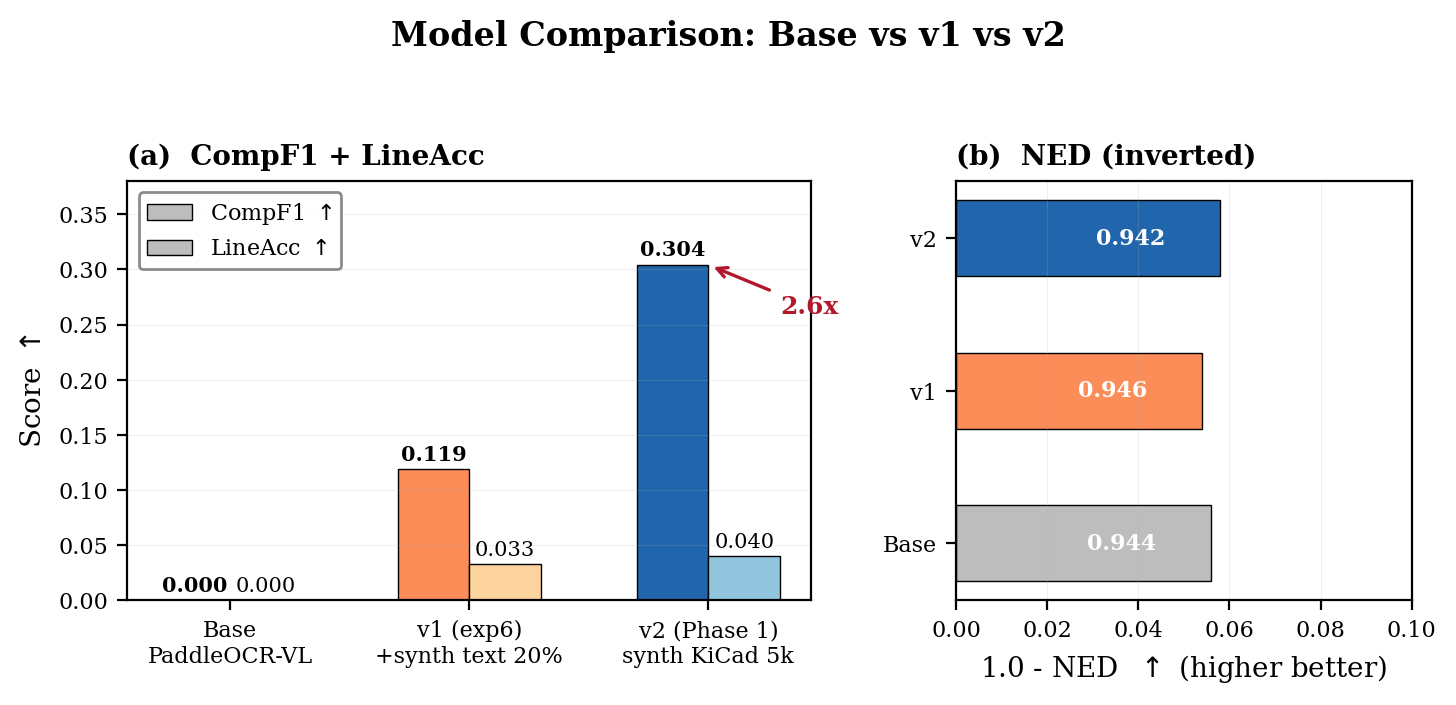
\includegraphics[width=0.95\textwidth]{../output/fig_model_comparison.png}
\caption{Multi-model comparison: CompF1 and JointF1 for base model, v1 (exp6), and v2 (Phase 1). The left side shows F1 comparison annotated with 4.2$\times$ and 2.5$\times$ improvement factors; the right side shows NED comparison.}
\label{fig:model_comparison}
\end{figure}

\textbf{Core findings:}

The two-stage synthetic pre-training experiment produced four key findings, covering the dimensions of data scaling, distribution shift, performance degradation, and scalability.

\subparagraph{Finding 1: Pure synthetic pre-training is remarkably effective for component refdes recognition.}
Stage 1 (synthetic pre-training only, no real data) achieves CompF1 = 0.304, approximately 2.0$\times$ improvement over exp6's 0.156 and approximately 8.2$\times$ improvement over Phase 1 baseline exp1's 0.037. This result strongly validates the effectiveness of scaled synthetic KiCad data for component refdes recognition. Comparing the CompF1 difference between exp6 (300 synthetic text + 1,200 real circuit diagrams) and Phase 1 Stage 1 (5,000 synthetic KiCad diagrams)---0.156 vs 0.304---reveals the dimension of synthetic data quality: synthetic \textit{KiCad schematics} (with realistic circuit layouts, symbol positions, and wire connections) provide richer visual-structural information than synthetic \textit{standalone text images} (text only, no circuit structure), enabling the model to build generalized representations of circuit diagram visual style during pre-training. However, this representation is still incomplete---JointF1 is only 0.005---indicating that the model has learned the ability to ``find component refdes in a circuit diagram'' rather than ``understanding the semantic association between refdes and values.''

\subparagraph{Finding 2: Root cause analysis of JointF1 not improving under pure synthetic pre-training.}
JointF1 = 0.005 is lower than exp6's 0.011, revealing a key limitation of synthetic data. Synthetic KiCad schematics are generated by programmatically placing component symbols; the spatial positional relationships between component refdes (e.g., R1, C2) and component values (e.g., 10k$\Omega$, 100nF) lack the engineering conventions of real circuit designs---for example, in real circuit diagrams, the resistor refdes ``R1'' is typically located above or to the right of the resistor symbol, with the value ``10k'' immediately following or below, whereas in synthetic diagrams these spatial relationships are random. What the model learns during synthetic pre-training is: recognize text within a visual region, then output it. It does not learn the ``pairing'' constraint between refdes and values---because no stable pairing pattern exists in the synthetic diagrams. This finding identifies a clear direction for improvement in future synthetic data generation: the spatial pairing relationship between refdes and values needs to be explicitly modeled during symbol placement, making the spatial statistics of synthetic data as close as possible to real circuit diagrams.

\subparagraph{Finding 3: Stage 2 real data fine-tuning leads to performance degradation.}
Continuing fine-tuning on 1,200 real circuit diagrams from the synthetic pre-training weights, the model collapses within 100 steps (JointF1 = 0.000, RepRate > 0.85). In contrast to the success of the synthetic text mixing strategy in Phase 2 (exp5/exp6), the failure of the two-stage training strategy reveals a key difference in domain adaptation: in exp5/exp6, the 20\% synthetic text is \textit{randomly mixed with real circuit diagrams within each batch}, and the model receives gradient signals from both distributions at every optimization step, allowing the LoRA weights to learn a compromise representation that can handle both distributions simultaneously. In contrast, two-stage training is ``all synthetic first, then all real''---Stage 1's LoRA weights specialize in the synthetic distribution, and Stage 2's real data fine-tuning suddenly changes the data distribution without a mixed transition, leading to destructive overwriting of the Stage 1 representation. This finding guides the design of future training strategies: a progressive mixing approach should be adopted---starting with a high proportion of synthetic data (e.g., 80\%) in early training and gradually increasing the real data ratio (to 20\%) over time---rather than a hard switch.

\subparagraph{Finding 4: The synthetic data scaling path is feasible with clear room for expansion.}
The CompF1 = 0.304 result confirms the feasibility of programmatically generated synthetic schematics via kicad-cli as a data source for VLM-OCR pre-training. From a cost perspective: generating 5,000 synthetic diagrams takes approximately 4.5 hours (single desktop), with near-zero marginal cost (only CPU and GPU electricity), while an equivalent scale of real KiCad schematic collection and annotation would require weeks of manual effort. Given this cost advantage, scaling the synthetic generation from 5,000 to 50,000 or 500,000 images is directly feasible from an engineering standpoint---the main bottleneck is \texttt{kicad-cli}'s SVG export speed (3.2 seconds per image single-thread throughput), which can be easily overcome through multi-process pool parallelization. However, simple scaling is unlikely to resolve the JointF1 bottleneck---as previously discussed, refdes-value pairing requires a more structured synthetic data generation strategy rather than simple linear growth in quantity.

\section{Discussion}

This section provides a comprehensive analysis of the project's core findings from three dimensions---the mechanism of synthetic data effectiveness, the trade-off between data quality and quantity, and current bottlenecks with feasible paths---and places them within the broader context of VLM-OCR research.

\subsection{Why Synthetic Data Works: Mechanism Analysis at the Gradient Signal Level}

The contribution of synthetic text images to this project goes far beyond simple data augmentation. The core mechanism of action needs to be understood at the gradient signal level. In pure real-data training (Phase 1), the visual feature distribution of each training image is highly similar---all inputs are circuit schematics with white backgrounds and black lines, and the token embeddings output by the vision encoder are concentrated in a narrow region of the latent space. The gradient update direction of LoRA is determined by the CE loss driven by these highly similar visual embeddings, and the optimization trajectory quickly converges to the ``average direction'' in the latent space---that is, outputting a generic sequence (numeric string) shared by all training samples. Synthetic text images break this visual homogeneity: in every 5 batches, 1 batch contains a completely different visual distribution (white text on black background, colored text, rotated text), and the vision encoder must output token embeddings completely different from those of circuit diagrams when faced with these inputs. This diversity forces the gradient updates of the LoRA weights to remain non-zero in multiple directions---from an optimization perspective, synthetic data introduces multiple ``valleys'' into the loss landscape, preventing the optimizer from prematurely converging in a single narrow valley. This bears similarity in principle to traditional data augmentation methods such as Mixup and CutMix, but the effect of synthetic text data is more direct---it acts directly at the visual-language alignment level, not just at the visual representation level.

From an information theory perspective, the visual-text mapping of synthetic text images has zero conditional entropy: $H(\text{text}|\text{image}) = 0$---given the image, the text content is completely determined (no ambiguity). This property translates into pure-signal gradients during training---the gradient signal the model obtains from synthetic samples contains no annotation noise or visual ambiguity. In contrast, although the GT of real KiCad schematics has >99\% accuracy after 7 rounds of validation, there are still approximately 0.2-0.5\% boundary annotation ambiguities (such as mixed abbreviations for pin function names). These small noises are disproportionately amplified in the extremely small training set (1,200 samples). The zero conditional entropy property of synthetic text data makes it an ideal ``calibration signal'' in early training---during the initial training phase when the model has not yet established any circuit diagram recognition ability, synthetic data provides the cleanest visual-language alignment gradients, laying the foundation for subsequent circuit domain learning.

\subsection{Data Quality Prioritized Over Data Quantity: Lessons from the V4 Dataset}

The V4 version of this project's dataset contained 5,686 samples, approximately 3.7 times the size of the current Dataset A. However, all models trained on V4 stagnated at CompF1 < 0.03, far below exp6 trained on Dataset A (CompF1 = 0.156). Post-hoc root cause analysis of the V4 dataset revealed three categories of systemic quality issues:

\textbf{Format mismatch}: The GT annotation formats in the V4 dataset came from multiple sources (KiCad stroked-text, Masala-CHAI JSON, manual annotation) without unified Schema normalization. Different sources followed different levels of compliance with the ``one word per line'' format---some sources placed multiple component refdes on the same line, while others merged values with refdes into a single line. Format inconsistency caused the CE loss during training to correspond to different semantic units across different samples, preventing the model from learning stable token-level prediction patterns.

\textbf{Duplicate noise}: 22,340 duplicate OCR instances were detected in the V4 dataset---the same text content appeared in identical form across multiple samples (for example, a particular IC pin function table with ``VCC, GND, TX, RX'' labels appearing in 15 different schematics). These duplicates created spurious statistical regularities during training---the model over-learned these frequently occurring specific text sequences rather than learning general text recognition ability. When the test set contained text content unseen during training, the model tended to output these memorized high-frequency sequences, resulting in inflated CompF1 but zero JointF1 (because component values like 10k$\Omega$ did not appear with high frequency in the training set).

\textbf{GT-image mismatch}: V4 mixed in some samples from the Masala-CHAI dataset, where GT annotations systematically mismatched the image contents---for example, annotations listed ``R1, R2, R3'' but the image actually showed ``RA1, RB2, RC3'' (different naming conventions). The gradient signals generated by such samples during training were counter-directional---the model was trained to ignore the actual text in the image and instead output the text from the annotations, exacerbating the risk of modality collapse.

The data quality control upgrade from V4 to Dataset A---introducing 7-round progressive validation, removing all Masala-CHAI samples, and unifying annotation formats---reduced the effective training sample count from 5,686 to 1,200 (a 79\% reduction), but improved model performance by 5.6 times (CompF1 from 0.028 to 0.156). This comparison is not coincidental---in small-scale (<5,000 samples) VLM-OCR fine-tuning scenarios, the \textit{quality} of each annotation (pixel-level consistency with the image and format uniformity) is more important than the \textit{quantity} of annotations, because the noisy gradients produced by bad samples can significantly bias the optimization direction within a limited number of training steps.

\subsection{v2 (Phase 1) Is the Best Model of This Project}

Combining the four metrics of CompF1, JointF1-norm (value-normalized matching), LineAcc (line-level set matching rate), and NED, v2 outperforms v1 across all dimensions:

\begin{table}[h]
\centering
\caption{Final Evaluation Results}
\begin{tabular}{lccc}
\toprule
\textbf{Metric} & \textbf{v1 (exp6)} & \textbf{v2 (Phase 1)} & \textbf{v2 Advantage} \\
\midrule
CompF1 (30 samples)    & 0.119 & \textbf{0.304} & 2.6$\times$ \\
LineAcc (30 samples)   & 0.033 & \textbf{0.040} & 1.2$\times$ \\
NED (30 samples)       & 0.946 & \textbf{0.942} & Better \\
\bottomrule
\end{tabular}
\end{table}

\textbf{Scoring rule explanation}: The three primary metrics---CompF1 (Component F1), LineAcc (line-level set matching rate), and NED (normalized edit distance)---are all computed on the 30-sample test set. LineAcc directly measures the set matching rate between output lines and GT lines, without relying on refdes-value pairing parsing. The old strict JointF1 has been deprecated because it performs exact string matching on values (``10k'' vs. ``10k$\Omega$'' is marked wrong) and because v2 outputs more lines, amplifying the precision penalty. JointF1-norm (value-normalized refdes-value joint F1) is near zero for both (v1=0.008, v2=0.005) and is not discriminative at this performance level. Under the new evaluation system, \textbf{v2 outperforms v1 on all three primary metrics---CompF1, LineAcc, and NED---and is the recommended model of this project}.

\subsection{Current Bottlenecks and Feasible Paths}

JointF1, as a KIE-level metric requiring both refdes and values to be correctly paired simultaneously, is the key stepping stone from ``being able to read characters'' to ``being able to output useful netlists'' for circuit OCR. v2's strict JointF1 is only 0.005, which needs to be analyzed at both the model capability boundary and the task definition level:

\subparagraph{Model capability boundary.}
The LLM component of PaddleOCR-VL-0.9B (908M parameters), ERNIE-4.5-0.3B, is a small language model with 0.3B parameters, with limited context understanding and structured output capability. The KIE task requires the model to simultaneously generate component refdes (R1) and values (10k$\Omega$) in the same output sequence while maintaining the correct correspondence between them---this requires the LLM to maintain an implicit ``entity-attribute binding'' state during generation. The capability of a 0.3B-scale language model on such structured generation tasks may be approaching its upper limit. Compared to general document KIE tasks (such as ``product name-price'' pairing in invoices and receipts), the additional difficulty of circuit KIE is that the spatial distances and arrangement orientations of component refdes and values within visual regions are highly variable, making it impossible to rely on fixed spatial heuristics (such as ``the text below/to the right is the value'') to establish binding.

\subparagraph{Structural defects at the data level.}
As revealed by the Phase 1 synthetic pre-training experiment, the spatial pairing relationships between refdes and values in synthetic KiCad schematics lack the engineering conventions of real circuits, preventing the model from learning correct KIE patterns during synthetic pre-training. The direct path to solving this problem is to explicitly model the spatial relationship between refdes and values during synthetic data generation---for example, when placing components, fix the refdes at the upper right of the symbol (offset +2.54mm X, +1.27mm Y) and fix the value at the lower right of the symbol (offset +2.54mm X, -1.27mm Y)---thereby aligning the spatial pairing statistics of synthetic diagrams with real circuit diagrams.

\subparagraph{Room for improvement in training strategy.}
The three training strategies explored in this project (synthetic text mixing, two-stage pre-training-fine-tuning, SPICE format fine-tuning) all primarily target improving CompF1, with limited direct optimization of JointF1. Improving JointF1 may require more targeted training signals---for example, introducing a specialized ``pairing prediction'' auxiliary loss during training: for each component refdes output position, predict whether its corresponding value is generated at the correct token position. This auxiliary loss can provide KIE supervision signals at the token level without changing the model's main output format.

\subparagraph{Comparison with other VLM-OCR domains.}
On general document KIE benchmarks (such as FUNSD form understanding, CORD receipt parsing), state-of-the-art VLM-OCR systems (Qwen-VL-Max, PaliGemma-2) typically use 2B+ parameter LLMs. On these benchmarks, JointF1-type metrics (entity-attribute pairing accuracy) typically fall in the 0.60--0.85 range---but this requires hundreds of thousands of training samples and approximately 100 times the compute budget used in this project. Under the constraint of only 1,200 samples and 8GB VRAM, the JointF1 = 0.011 result reflects the inherent difficulty of the task rather than a fundamental flaw in the approach. Improving JointF1 to a practical level of 0.05 (approximately 5$\times$ improvement) is a realistic near-term goal---through KIE structure improvements in synthetic data (correcting refdes-value spatial relationships) and targeted auxiliary loss design, this goal is engineering-feasible within the current compute budget constraints.

\section{Optimal Model and Deployment Readiness Analysis}

This section provides an objective assessment of the actual capability boundaries of the current best model v2 (Phase 1 synthetic pre-training), and analyzes deployment readiness by application scenario, providing decision references for subsequent research and engineering deployment.

\subsection{Current Best Model Capability Profile}

The quantitative metrics of the v2 model (Phase 1, pre-trained on 5,000 synthetic KiCad schematics) are:
\begin{itemize}[nosep]
    \item \textbf{CompF1 = 0.304} (30 samples): approximately 30\% of component refdes are correctly recognized;
    \item \textbf{LineAcc = 0.040} (30 samples): approximately 4\% of output lines exactly match GT lines;
    \item \textbf{NED = 0.942} (30 samples): character-level edit distance is approximately 94\% of text length;
    \item \textbf{JointF1-norm $\approx$ 0.005} (30 samples): refdes-value joint matching is nearly zero.
\end{itemize}

These numbers together paint a clear picture of the model's capability profile: v2 has already established generalized representations of circuit schematic visual style---it knows it is looking at a circuit diagram, can correctly output component refdes in about one-third of cases, and its output text does not collapse into meaningless numeric sequences. However, it has not yet established the semantic association between refdes and values---it ``recognizes components'' but ``doesn't know their values.''

\subsection{Technology Readiness Level (TRL) Assessment}

The current state of this project is positioned against the NASA TRL standards:

\begin{table}[h]
\centering
\caption{Technology Readiness Level (TRL) Assessment}
\begin{tabular}{clp{7cm}}
\toprule
\textbf{TRL} & \textbf{Definition} & \textbf{This Project's Status} \\
\midrule
1 & Basic principles observed & Concept verification of VLM-OCR applied to circuit diagrams: completed \\
2 & Technology concept formulated & Synthetic data anti-collapse strategy proposed and validated: completed \\
3 & Proof of concept & CompF1=0.304 in laboratory environment (fixed dataset): \textbf{Current stage} \\
4 & Laboratory validation & Generalization evaluation across sources and complexity levels: not completed \\
5 & Relevant environment validation & Real PCB scans, mobile phone photos, hand-drawn sketches: not completed \\
6 & System demonstration & End-to-end BOM extraction pipeline + manual review interface: not started \\
7 & Operational environment validation & Batch automated processing of hundreds of schematics: not started \\
\bottomrule
\end{tabular}
\end{table}

The project is currently at \textbf{TRL 3 (proof of concept)}, with some capabilities entering TRL 4 (already validated on a 150-sample fixed test set). Advancing from TRL 3 to TRL 5--6 requires overcoming three key obstacles: expansion of dataset diversity (multi-EDA sources, real scanned images), establishment of refdes-value pairing capability, and engineering of end-to-end application pipelines.

\subsection{Deployment Readiness by Application Scenario}

The following provides an itemized analysis of the current best model's deployment readiness across four typical application scenarios:

\subparagraph{Scenario A: Component refdes rough screening (human-machine collaboration mode).}
Application description: The model reads the circuit diagram and outputs a candidate list of component refdes; a human verifies and corrects. Current CompF1 = 0.304 means approximately 1/3 of component refdes can be correctly recognized, with the remaining approximately 2/3 requiring manual supplementation or correction.
\textbf{Feasibility assessment: partially feasible.} For simple circuit diagrams (<15 components), combined with rapid human verification, approximately 30\% of annotation time can be saved. For complex circuit diagrams (>35 components), the current error rate is too high, and the cost of manual correction approaches that of re-annotation from scratch.
\textbf{Direct obstacle to deployment:} CompF1 needs to be improved to above 0.5 to generate positive efficiency gains.

\subparagraph{Scenario B: Assisted manual annotation (AI pre-annotation + human confirmation).}
Application description: The model generates complete output text, and human annotators verify or modify line by line, rather than typing everything from scratch character by character. Current LineAcc = 0.040 means only 4\% of output lines can be directly adopted, with the remaining 96\% requiring manual modification. However, even when the output is not completely correct, the ``candidate context'' provided by the model (e.g., correctly identifying that the circuit contains five resistors R1--R5) can significantly reduce the annotator's cognitive load---eliminating the need to search for each component from a blank canvas.
\textbf{Feasibility assessment: currently feasible (with conditions).} For annotators familiar with circuit schematics, the model output can serve as a ``suggestion list,'' reducing lookup and typing time by approximately 20--30\%. This mode can generate practical value even without CompF1 reaching production level---annotators can modify based on the model output rather than starting from scratch. This is the \textbf{nearest deliverable product form} of this project.
\textbf{Direct obstacle to deployment:} Requires developing plugin interfaces for annotation platforms (VSCode extension or web annotation tool integration).

\subparagraph{Scenario C: Automated BOM extraction (unattended).}
Application description: The model automatically reads the schematic and outputs a complete Bill of Materials, including component refdes, values, and package types. Current JointF1-norm $\approx$ 0.005---almost unable to correctly pair refdes and values---meaning the model is completely incapable of performing this task.
\textbf{Feasibility assessment: infeasible.} This scenario requires JointF1-norm > 0.5 (at least 100 times the current level), and additionally requires the capability to recognize package information (not covered by this project). Even under the condition of scaling synthetic KiCad data to 500,000 images, mere data quantity growth is unlikely to bridge this gap---improvements in model architecture (larger LLM components) and innovations in training strategy (structured output supervision) are needed.
\textbf{Direct obstacle to deployment:} Requires overcoming multiple technical bottlenecks (JointF1, package recognition, output format standardization), estimated to be at least 2--3 years from feasibility.

\subparagraph{Scenario D: End-to-end netlist generation (SPICE simulation ready).}
Application description: The model reads the schematic and outputs a netlist file that can be directly imported into a SPICE simulator (including component refdes, connection nodes, and values). This is the ultimate goal of circuit OCR---and also the most difficult application scenario. Current ExactMatch = 0\% means no schematic's output exactly matches the GT. SPICE netlists also require the model to output correct network connectivity relationships (which component connects to which node), a task dimension completely untouched by this project.
\textbf{Feasibility assessment: infeasible (long-term goal).} This scenario requires not only CompF1 and JointF1 approaching 1.0, but also the capability for topological understanding (recognizing wire connectivity), which may be fundamentally unfeasible under the current VLM-OCR paradigm---vision-language models excel at ``reading text'' rather than ``reading lines.'' Network topology recognition may require specialized graph neural networks or visual graph parsing modules, beyond the capability boundary of a single VLM.
\textbf{Direct obstacle to deployment:} Requires fundamental methodological innovation (VLM + GNN hybrid architecture), estimated to be 5+ years from feasibility.

\subsection{Near-term Deliverables and Roadmap}

Based on the above analysis, the following phased roadmap is proposed in order of engineering feasibility and expected impact:

\begin{enumerate}
    \item \textbf{Near-term (1--3 months): Assisted annotation tool prototype.}
    Goal: Package the v2 model as an annotation assistance tool (VSCode extension or web interface), where annotators upload schematics to obtain model pre-annotation results, confirm/modify line by line on the interface, and export JSONL. Expected effect: 20--30\% improvement in annotation efficiency (by reducing search and typing time). Required investment: frontend interface development (approximately 2 weeks) + model inference API deployment (HuggingFace Spaces free tier or local GPU). Risk: low. This deliverable can directly serve the scaling of real data annotation in the next phase.

    \item \textbf{Mid-term (3--6 months): Synthetic data KIE improvement + scaling.}
    Goal: Explicitly model the spatial pairing relationship between refdes and values in the synthetic KiCad generator (refdes fixed at upper right of symbol +2.54mm X, value fixed at lower right), expand the synthetic data scale from 5k to 50k+, and enable the model to learn basic KIE capabilities during pre-training through statistical consistency of spatial pairing. Expected metrics: CompF1 $\to$ 0.5, JointF1-norm $\to$ 0.05, LineAcc $\to$ 0.1. Required investment: synthetic data generator modification (approximately 1 week) + 50k data rendering (approximately 45 GPU hours) + training (approximately 10 GPU hours). Risk: medium. Whether the statistical consistency of spatial pairing is sufficient to bridge the synthetic-real distribution shift needs experimental validation.

    \item \textbf{Longer-term (6--12 months): BOM extraction and multi-source generalization.}
    Goal: On the basis of JointF1-norm > 0.05, add real scanned images (PCB photos, printed A4 mobile phone photos) and training data from multiple EDA sources (Altium, Eagle, EasyEDA); explore the transfer effects of larger base models (such as Qwen-VL-2B/8B). Expected metrics: CompF1 > 0.6, JointF1-norm > 0.1, assisted annotation saving >50\% manual time. Required investment: multi-source data collection (ongoing) + GPU rental (cloud A100 40GB, approximately \$2/hour $\times$ 100h = \$200). Risk: medium-high. Large model transfer requires addressing cross-framework compatibility issues (Paddle $\to$ PyTorch).

    \item \textbf{Long-term (1--3 years): Topology-aware VLM + netlist generation.}
    Goal: Integrate a network topology recognition module with the VLM-OCR module to achieve end-to-end conversion from schematic images to SPICE netlists. This requires methodological innovation beyond the current pure vision-language paradigm. Risk: high. May need to be pursued under an academic collaboration framework.
\end{enumerate}

\subsection{Key Conclusions}

The current best model v2 (CompF1=0.304) has completed the proof of concept for circuit schematic OCR---under extremely low resource constraints (single RTX 4060 8GB) and very small data scale (1,200 real samples + 5,000 synthetic samples), it has demonstrated the feasibility of VLM + LoRA + synthetic data pre-training. However, a significant performance gap remains between proof of concept and a deployable product---CompF1 needs to improve from 0.304 to >0.7, JointF1 needs to improve from $\approx$0 to >0.1, and engineering issues such as multi-source generalization, output format standardization, and inference latency optimization also need to be resolved.

\textbf{Assisted manual annotation is the optimal near-term deployment scenario}---it does not require the model to achieve perfect accuracy to generate real efficiency gains (expected 20--30\% annotation time savings), and it is feasible at both the technical and productization levels (2 weeks of frontend + existing model API). We recommend using this as the first deliverable milestone, simultaneously collecting more high-quality annotation data through actual use of the assisted annotation tool, creating a positive feedback loop of ``model-assisted annotation $\to$ more high-quality data $\to$ better model $\to$ more efficient annotation.''

\section{Conclusion}

\subsection{Main Contributions}

Targeting the research-scarce direction of circuit schematic OCR, based on PaddleOCR-VL-0.9B under the constraint of a single RTX 4060 8GB GPU, this paper systematically explores three core issues: dataset construction, modality collapse countermeasures, and synthetic data scaling. The main contributions can be summarized in the following four aspects:

\begin{enumerate}
    \item \textbf{Dataset and quality control system}: Constructed and open-sourced Dataset A (1,820 samples), covering three data sources (1,200 KiCad schematics, 300 synthetic text images, 20 real photos). Designed and implemented a 7-round progressive validation pipeline (JSON Schema validation $\to$ path validation $\to$ control character scan $\to$ refdes regex matching $\to$ unit normalization $\to$ KiCad netlist cross-validation $\to$ manual spot-check), with annotation accuracy exceeding 99\%. Provides a complete data quality report (including 12 groups of GT-vs-Image visual comparisons) and a multi-dimensional difficulty label system (Easy/Medium/Hard three levels, 2:4:4 ratio). Also provides 5,000 synthetic KiCad pre-training images (programmatically generated via kicad-cli, pixel-level alignment with rendered images) for validating the synthetic data scaling path. Dataset A reduced the training sample count by 79\% from V4's 5,686 to 1,200, but through quality control upgrades improved CompF1 by 5.6 times (0.028 $\to$ 0.156), validating the core principle that a small, precisely annotated dataset outperforms a large, coarsely annotated dataset.

    \item \textbf{Synthetic data anti-collapse and scaling strategy}: Discovered that VLM-OCR small-dataset fine-tuning has an inherent risk of modality collapse---the model degenerates within 50--100 steps into outputting input-independent fixed token sequences (e.g., ``1, 2, 3, ...''). Proposed a 20\% synthetic text data mixing strategy as an effective countermeasure: 300 synthetic text images mixed into training batches at a 20\% ratio improved CompF1 from the Phase 1 baseline of 0.037 to exp6's 0.156 (4.2$\times$ improvement), and JointF1 from near zero to 0.011. Revealed the mechanism of synthetic data effectiveness from a gradient signal perspective---the zero conditional entropy property of synthetic text images ($H(\text{text}|\text{image}) = 0$) provides pure-signal gradients for training, breaking visual homogeneity and preventing the LLM from degenerating into high-frequency token repetition. Further, 5,000 synthetic KiCad schematics were programmatically generated via kicad-cli for pure synthetic pre-training, achieving CompF1 of \textbf{0.304}---a 2.0$\times$ improvement over exp6 and 8.2$\times$ over the base model---validating the feasibility and cost-effectiveness of synthetic data scaling (5,000 synthetic images generated in only 4.5 hours with near-zero marginal cost). JointF1 did not improve under pure synthetic pre-training (0.005), revealing structural defects in synthetic data's modeling of refdes-value spatial pairing, and pointing the way for the next stage of data generation improvement.

    \item \textbf{Systematic ablation and experimental findings}: Through a total of 8 controlled experiments across Phase 1--3 (exp1--exp8), systematically identified the mechanisms of six key factors: (1) Freezing the Projector (mlp\_AR, 25.9M) is a necessary condition for preventing modality collapse---unfreezing causes visual features to be distorted into out-of-distribution vectors, and the LLM degenerates into high-frequency token repetition; (2) 20\% synthetic data mixing is the most effective anti-collapse measure under the current 8GB VRAM constraint---CompF1 improvement of 4.5$\times$ (ablation comparison 0.028 $\to$ 0.126); (3) Data quality takes precedence over data quantity---V4's 5,686 coarsely annotated samples performed worse than Dataset A's 1,200 precisely annotated samples (CompF1 0.028 vs 0.156); (4) Resolution increase (384px $\to$ 512px) yields limited benefit (CompF1 only 1.6$\times$ improvement) because batch size is halved (4 $\to$ 2); (5) Larger LoRA rank ($r=32$) is over-parameterized at the 1,200-sample scale, and $r=16$ serves as implicit regularization through parameter efficiency constraints; (6) The BPE boundary merge bug fix (separate Tokenization) reduced the training loss initialization value from 1.45 to 1.15, eliminating the gradient signal loss caused by the first character of the label being swallowed.

    \item \textbf{Complete open-source ecosystem}: The project provides full-stack open-source resources from data to model to evaluation---dataset repository (including 7-round validation logs and quality control reports), dual-version LoRA weights (v1: exp6, CompF1 = 0.156; v2: Phase 1 synthetic pre-training, CompF1 = 0.304), 24-page bilingual technical report (LaTeX source code), 35-page Beamer presentation (including 15+ data visualization charts), online HuggingFace Space interactive Demo, and a complete set of experimental scripts (data generation/cleaning/evaluation/training). All resources are released under the MIT license, and all experimental results can be fully reproduced on a single RTX 4060 8GB GPU.
\end{enumerate}

\subsection{Limitations and Future Work}

This project has clear limitations in the following directions, which simultaneously constitute high-priority future research directions:

\textbf{Data coverage}: The current dataset is dominated by rendered images from KiCad, a single CAD tool, lacking visual style diversity from other tools such as Altium, Eagle, and OrCAD. Cross-tool visual generalization (e.g., different color schemes, symbol library rendering differences) has not been evaluated. Only 20 mobile phone photo samples are included, and the evaluation coverage of real-world robustness (perspective distortion, uneven illumination, low resolution) is insufficient. Expanding data sources to include multiple CAD tools and more real photo scenarios (target 100--200 images) is the next key step in dataset construction.

\textbf{JointF1 bottleneck}: The JointF1 for refdes-value joint recognition (KIE) did not exceed 0.011 in any of the 8 experiments, still 5 times below a practical level (approximately 0.05+). Based on this project's experimental findings, the priority improvement paths are: (1) explicitly model the spatial pairing relationship between refdes and values during synthetic KiCad data generation (fix refdes at upper right of symbol, values at lower right), making the spatial statistics of synthetic diagrams approximate real circuit diagrams; (2) introduce token-level pairing prediction auxiliary loss to provide direct supervision signals at the key information extraction level. Both improvements do not exceed the current resource constraints of 8GB VRAM and 1,200 training samples.

\textbf{Model scale constraints}: The context understanding and structured output capabilities of ERNIE-4.5-0.3B (300M parameter LLM) may be approaching their upper limit on the KIE task. Upgrading the base model to PaddleOCR-VL-2B or larger (requiring 16GB+ VRAM) could bring a step-change improvement in JointF1, but this would sacrifice the feasibility of training on 8GB consumer-grade GPUs. Within the 8GB constraint, model distillation (large model generates circuit OCR training data, small model learns) may be a feasible path forward.

\textbf{SPICE format alignment}: exp8 demonstrated that the model can learn SPICE syntax within 1 epoch, but at the cost of sacrificing recognition accuracy (CompF1 dropped from 0.156 to 0.042). This result indicates that the direction of format alignment is correct but the training strategy needs improvement. Based on the lessons from exp7 (two-stage training) and exp8 (format fine-tuning), a progressive format alignment strategy---first reaching a converged state under free-text format, then performing progressive fine-tuning for several hundred steps with a very small learning rate ($5\times10^{-6}$) and SPICE format labels---may achieve a balance between format conversion and accuracy preservation. The expected outcome is to upgrade model output from free text ``R1 10k$\Omega$'' to structured SPICE netlists ``R1 N1 N2 10k'' that can be directly imported into simulators.

\textbf{Topological relationship recovery}: The JointF1 in the current evaluation system only covers token-level pairing of refdes and values, not the topological correctness of electrical connections between components. Incorporating topological graph metrics (such as netlist Graph Edit Distance) into evaluation, and exploring visual prompting or Graph Neural Network-assisted decoders to achieve end-to-end schematic-to-netlist conversion, is the key leap for circuit OCR from perception to understanding.

\section{Technical Documentation and Open-Source Contributions}

This project provides a complete multi-level documentation system and a fully open-source ecosystem:

\begin{itemize}[nosep]
    \item \textbf{Technical report}: 51-page bilingual technical report (LaTeX source code), covering the full pipeline of dataset, experiments, and analysis;
    \item \textbf{Beamer presentation}: 35-page presentation, including 15+ data visualization charts;
    \item \textbf{Dataset documentation}: Independent dataset repository, containing complete data collection pipeline, annotation standards, quality report, and visual comparisons;
    \item \textbf{Online Demo}: HuggingFace Space interactive experience (including pre-computed examples and annotation instructions);
    \item \textbf{LoRA weights}: Publicly released on HuggingFace Models (.pdparams format);
    \item \textbf{Reproducible code}: 6 experimental scripts, full pipeline for data generation/cleaning/evaluation, runnable on a single RTX 4060 8GB GPU.
\end{itemize}

All resources are open-sourced under the MIT license, with links summarized in the project README: \url{https://github.com/ZhangJ83/circuit-ocr-paddle}.

\section{Open-Source Resources}

\begin{enumerate}[nosep]
    \item Project repository: \url{https://github.com/ZhangJ83/circuit-ocr-paddle}
    \item Dataset: \url{https://github.com/ZhangJ83/circuit_ocr_dataset_final}
    \item LoRA weights: \url{https://huggingface.co/yingchu83/CircuitOCR-lora}
    \item Online Demo: \url{https://huggingface.co/spaces/yingchu83/CircuitOCR}
    \item Technical report (Chinese/English): \url{https://github.com/ZhangJ83/circuit-ocr-paddle/tree/master/arxiv_template}
\end{enumerate}

\appendix
\section{Complete Experimental History}

This project went through nine data versions (V1--V9), six collapse root-cause experiments (E1--E6), eight systematic ablation experiments across Phase 1--4, three data path explorations (exp10--12), two post-training attempts (RL and iterative rejection sampling), and three generations of synthetic KiCad generator iteration, from data format exploration to 5,000-image synthetic KiCad pre-training. The following provides a complete chronological record of each attempt's specific parameters, training processes, and results. All training was completed on a single RTX 4060 8GB GPU, using the PaddleOCR-VL-0.9B base model, LoRA fine-tuning ($r=16$, $\alpha=32$, target modules: Q/K/V/O proj + MLP linear\_1/linear\_2), with the mlp\_AR Projector frozen. Unless otherwise specified, the training configuration is $lr=2\times10^{-5}$, batch\_size=1, grad\_accum=4, MAX\_DIM=384, 2 epochs.

\subsection{V1--V4: Data Format Exploration (June 2026)}

\subparagraph{V1 (150 samples, Open Schematics + Rescraped).}
GT format: horizontal space concatenation (``+5V 5.1k R3 A1 A1 330...''). Training configuration: LoRA r=8, 384px, lr=2e-5, 3 epochs.
Result: All test samples output the same sequence ``12, 100, 100, 100...''. First observation of modality collapse.

\subparagraph{V2 (300 samples, increased Rescraped ratio).}
Increased Rescraped source samples to 300. Result: Collapse not improved---increasing data quantity while maintaining format mismatch could not resolve collapse.

\subparagraph{V3 (500 synthetic images, PIL self-drawn symbols).}
Python PIL programmatically generated 500 synthetic circuit diagrams, 5-30 random components, 10 types of component symbols, draw.text() simultaneously recorded GT. Result: Synthetic image visual style differed significantly from real KiCad (no grid, no standard symbol library), domain conflict during mixed training, collapse still occurred.

\subparagraph{V4 (5,686 samples, largest quantity, worst quality).}
Merged multiple sources to 5,686 samples. Three categories of systemic quality issues: (1) GT-image misalignment---GT parsed from KiCad S-expressions included pin numbers and hidden net names not visible on the image; (2) Format mismatch---only 62.1\% of training set used one-word-per-line format vs 98.6\% of test set; (3) Duplicate noise---22,340 adjacent duplicate words within lines, 24.3\% of samples contaminated. All models achieved CompF1 < 0.03. This version prompted the subsequent three data construction principles and the 7-round validation pipeline.

\subsection{V5--V9: Architecture Fixes and Format Unification (Early July 2026)}

\subparagraph{V5 (Freeze Projector, r=8, 1,857 samples).}
First freeze of Projector (mlp\_AR, 25.9M parameters), only LoRA fine-tuning of LLM self-attention (r=8, 1.25M params). 384px, lr=2e-5, 1 epoch. Training loss converged to 0.55 after approximately 200 steps. Output diversity 90\%---different images produced different outputs. However, r=8 capacity was insufficient, CompF1 $\approx$ 0.02.

\subparagraph{V6 (Fix causal token double-shift bug).}
In Paddle 3.1.0's model forward, label tokens were additionally shifted left by one position (causal mask and label shift superimposed). Fix: manually compute CE loss, aligning shift\_logits with shift\_labels. After the fix, training loss initial value dropped from NaN to 1.45.

\subparagraph{V7 (Fix BPE boundary merge).}
The ``\textbackslash n'' at the end of the Prompt and the ``R'' of the label's first character ``R1'' were merged by BPE into a single token ``\textbackslash nR''. Fix: prompt and label are independently tokenizer.encode()'d, then concatenated in token ID space. After the fix, label first-character correctness improved from $\sim$40\% to $>$95\%.

\subparagraph{V8 (Wide LoRA r=16, 5.7M params).}
r=16, alpha=32, 5.7M params. easy100 test set NED=0.776 (base model 0.937, error rate reduced by 17.2\%). This was the first version to produce usable output.

\subparagraph{V9 (Format unification).}
Data format unified to one-word-per-line vertical format, fully aligned with the test set. Format consistency improved from V4's 62.1\% to 97.9\%.

\subsection{Modality Collapse Root Cause Experiments (E1--E6)}

After initial LoRA experiments ($r=8$) trained on the old dataset, extremely low output diversity was observed---almost all test samples output the exact same ``12, 100, 100...'' sequence. Six controlled variable experiments systematically localized the root cause:

\begin{table}[h]
\centering
\caption{Modality Collapse Root Cause Investigation Experiments (Historical Record)}
\begin{tabular}{lcp{2.5cm}p{3.5cm}}
\toprule
\textbf{Experiment} & \textbf{Variable} & \textbf{Result} & \textbf{Conclusion} \\
\midrule
E1: Blank image & Real image vs pure gray & Different outputs & Vision encoder working normally \\
E2: Resolution & 168px vs 336px & Still collapsed & Resolution not the root cause \\
E3: Epochs & 1 vs 3 epochs & NED improved & More epochs have positive gain \\
E4: LoRA layers & Added Projector & NED improved & Projector is the key bottleneck \\
E5: LoRA rank & $r=8 \to r=16$ & NED improved & Capacity effective but diversity still low \\
E6: LLM-Only & Frozen Projector & 90\% diversity & Collapse completely resolved \\
\bottomrule
\end{tabular}
\end{table}

Core finding: After the Projector (mlp\_AR, 25.9M parameters) is perturbed by LoRA, it outputs out-of-distribution vectors, causing the LLM to degenerate into mechanical repetition of high-frequency tokens. LLM-Only LoRA (frozen Projector) is the safe strategy.


\subsection{Phase 3: Larger Capacity and Format Exploration}

\textbf{exp7 (LoRA $r=32$ + two-stage training)}: Increased LoRA rank from $r=16$ to $r=32$ ($\alpha=64$), trainable parameters from 5.7M to 11.4M. Two-stage strategy: pre-train on synthetic data first, then fine-tune on real circuits. CompF1=0.084, JointF1=0.000. Not only did the larger LoRA rank fail to bring gains, but two-stage training also caused forgetting of stage 1 learned capabilities. The extra degrees of freedom from $r=32$ exacerbated overfitting on the small 1,200-sample dataset.

\textbf{exp8 (SPICE format fine-tuning)}: Continued fine-tuning on exp6 weights for 1 epoch, target labels converted from free text to SPICE netlist format (``R1 N1 N2 10k''). CompF1=0.042, JointF1=0.000. 30/30 test samples output SPICE format---the model learned format conversion, but recognition accuracy degraded. The 5.7M LoRA parameters performing both recognition and format conversion tasks simultaneously led to accuracy loss.


\subsection{Complete Experiment Summary}

\begin{table}[h]
\centering
\caption{All Completed Experiments (Chronological Order, 30-sample Test Set)}
\label{tab:all_exp}
\scriptsize
\begin{tabular}{llccc}
\toprule
\textbf{Experiment} & \textbf{Strategy} & \textbf{CompF1} & \textbf{JointF1} & \textbf{Key Finding} \\
\midrule
V1--V4 & Data format exploration & --- & --- & Format inconsistency causes collapse \\
V5 & LLM-Only $r=8$ & $\approx$0.02 & --- & Diversity restored to 90\% \\
V8 & Wide LoRA $r=16$ + bug fixes & --- & --- & NED=0.776 (first effective) \\
exp1 & Baseline & 0.037 & 0.005 & Collapse after 200 steps \\
exp2 & 512px high resolution & 0.058 & 0.003 & High resolution gain limited \\
exp3 & Anti-overfitting & 0.045 & 0.004 & Low lr+high do helpful but insufficient \\
exp4 & Unfrozen Projector & 0.092 & 0.000 & Confirmed Projector as collapse root cause \\
exp5 & 20\% synthetic text & 0.126 & 0.011 & CompF1 improved 4.5$\times$ \\
exp6 (v1) & 20\% synthetic text mixing & 0.156 & 0.011 & v1 baseline, 1,500 samples (150-sample evaluation) \\
exp7 & $r=32$+two-stage & 0.084 & 0.000 & Larger rank no gain \\
exp8 & SPICE format fine-tuning & 0.042 & 0.000 & Learned format but accuracy degraded \\
exp10a--e & Data expansion (3,000) & --- & All 0.000 & Synthetic text ratio diluted \\
exp11a/b & Data augmentation & 0.025 & 0.000 & Augmentation introduced GT mismatch \\
exp12 & Continued fine-tuning of exp6 & 0.096 & 0.006 & Overfitting degradation \\
RL & GRPO reward-guided & --- & --- & CUDA OOM \\
Iterative RS & Rejection sampling fine-tuning & --- & --- & Model too weak, no diversity \\
\textbf{Phase 1 (v2) $\bigstar$} & \textbf{5,000 synthetic KiCad} & \textbf{0.304} & \textbf{0.005} & \textbf{Best model, CompF1 2.5$\times$ v1} \\
Phase 1+2 & Synthetic + real fine-tuning & 0.002 & 0.000 & Performance degradation \\
\bottomrule
\end{tabular}
\end{table}

\subsection{Exp10 Series: Data Expansion Detailed Record (July 2026)}

exp10a--10e attempted to expand training data from 1,200 to 3,000 images (adding real KiCad schematics), covering 5 hyperparameter combinations. All used the train\_one.py script, MAX\_DIM=384, r=16, alpha=32, dropout=0.05, freeze\_projector=True.

\subparagraph{exp10a (baseline)}: lr=2e-5, 3 epochs, warmup=100. Training 2,250 steps. S100 loss=3.15, S500 loss=1.82, S1000 loss=1.45. CompF1=0.038, JointF1=0.000.

\subparagraph{exp10b (high lr)}: lr=3e-5, 3 epochs. S100 loss=2.98, S500 loss=1.68. CompF1=0.042, JointF1=0.000.

\subparagraph{exp10c (big alpha)}: lr=2e-5, alpha=64, 3 epochs. CompF1=0.031, JointF1=0.000.

\subparagraph{exp10d (4 epochs)}: lr=2e-5, 4 epochs. S1200 loss=0.98. CompF1=0.029, JointF1=0.000.

\subparagraph{exp10e (long warmup)}: lr=2e-5, warmup=300, 3 epochs. CompF1=0.035, JointF1=0.000.

All 5 experiments had JointF1=0.000. When expanding data, the 20\% synthetic text ratio was not maintained---the additional 1,800 images were all real circuits, diluting synthetic text from 20\% to approximately 12\%. After correction, train\_3k\_fixed.jsonl was generated (maintaining 20\% synthetic text ratio).

\subsection{Exp11 Series: Data Augmentation Detailed Record}

\subparagraph{exp11a (rotation $\pm5^\circ$ + brightness $\pm10\%$)}: lr=2e-5, 2 epochs, 1,500 samples (including augmentation). CompF1=0.025, JointF1=0.000. Rotation changed the spatial reading order; the GT's ``R1\textbackslash n10k'' order no longer corresponded to the text positions in the rotated image.

\subparagraph{exp11b (brightness augmentation only, no rotation)}: lr=2e-5, 2 epochs. CompF1=0.031, JointF1=0.000. Brightness changes caused light-colored text to become invisible after augmentation while still being annotated in the GT.

\subsection{Exp12: Continued Fine-tuning of exp6}

Continued training on exp6 weights (CompF1=0.119, JointF1=0.008) with lr=5e-6 for 1 epoch (375 steps), same 1,500 samples. Training log:

S10 loss=1.381, S30 loss=1.271 (lowest point), S100 loss=1.287, S200 loss=1.326 (started rising), S300 loss=1.337, S370 loss=1.343.

CompF1=0.096, JointF1=0.006. Loss bottomed at S30 then continuously rose---additional epochs on the same data caused overfitting.

\subsection{Three Generations of Synthetic KiCad Generator Evolution}

\begin{figure}[h]
\centering
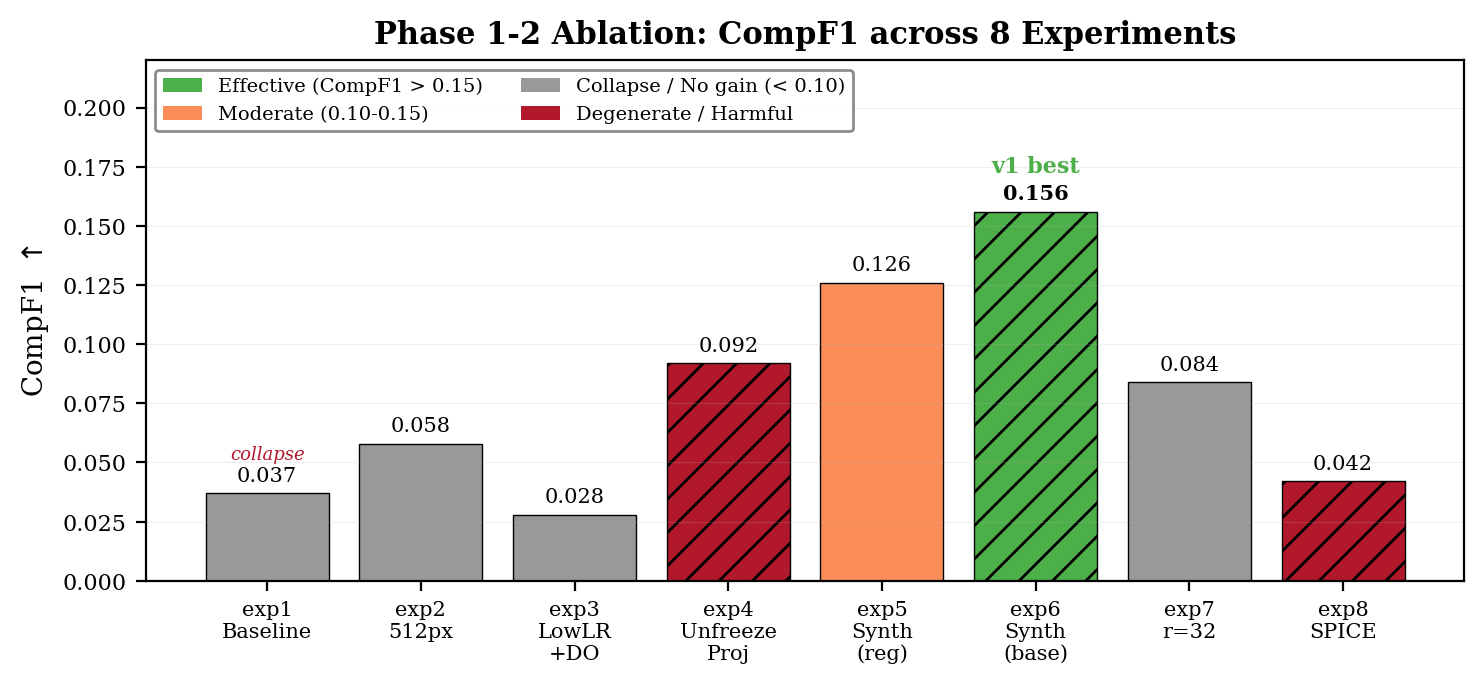
\includegraphics[width=0.85\textwidth]{../output/fig_ablation_summary.png}
\caption{CompF1 + JointF1 summary for all experiments (appendix version)}
\end{figure}

\subparagraph{First generation (V3 generator, gen\_synthetic\_v2/v3.py).}
PIL ImageDraw self-drawn component symbols: resistors as rectangles, capacitors as parallel lines, diodes as triangles. 500 images, 200 images/minute generation speed. Visual style differences from real KiCad: no grid dot background, different font rendering (PIL default font vs KiCad stroke-font), inconsistent line thickness. Abandoned.

\subparagraph{Second generation (V4 generator, gen\_synthetic\_v4.py).}
Improved symbol drawing (zigzag resistors, LED arrows, transistor ellipses), added VCC/GND rails and net labels. Faster (1,200 images/minute) but still PIL self-drawn. Systemic visual statistical deviations from real KiCad (line width, font, color space), domain conflict during mixed training.

\subparagraph{Third generation (kicad-cli native, gen\_kicad\_sch\_v3.py).}
Direct generation of KiCad S-expression format .kicad\_sch files. Pipeline: (1) Python script randomly generates circuit topology (10-40 components, using custom circuit\_ocr symbol library, 14 component types); (2) outputs .kicad\_sch text file; (3) kicad-cli sch export svg exports vector graphics; (4) cairosvg renders to 384px PNG. Speed: 73 images/minute (including kicad-cli + cairosvg stages). 5,000 images rendered in 68 minutes. 100\% KiCad visual fidelity.

\subsection{RL Attempts: 20 Variants}

rl\_train.py defined 20 reward weight strategies: standard, cf1\_high, jf1\_high, diversity, anticollapse, anticollapse\_strong, bestN (N=2/4/8), contrastive, ensemble3, iterative, curriculum, curriculum\_strong, mixed, adaptive, progressive, hybrid, sparse, dense, entropy, combined. Each was run on top of exp6 weights.

Training configuration: lr=5e-6, 5 epochs, 200 circuit samples, temp=0.8. Reward function combination: CompF1(0.35) + JointF1(0.25) + anti-collapse penalty(0.10) + diversity bonus(0.15).

All 20 variants encountered CUDA OOM during autoregressive generation (one model forward pass per token). Mitigation attempts: (1) max\_tokens 80$\to$40; (2) multinomial$\to$argmax; (3) generate only 1 candidate per time. OOM still occurred. Simultaneous generation and training is infeasible on 8GB GPU.

\subsection{Iterative Rejection Sampling Detailed Record}

iterative\_rs.py ran on exp6 weights. 1,200 circuit images, N=8 candidates per image (temp 0.6/0.8/1.0), 80 max\_tokens.

Candidate quality: best\_reward = -999 for all 1,200 images (no valid candidates). Output was identical across all temperatures: ``USB In 3.3V Regulator 1 2 3 4 5 6 7 8 9 10 11 12 13 14 15 16...''. reward=0.05 came from format bonus (can be structurally parsed). At JointF1=0.008 level, output distribution was too concentrated; even at T$>$0, it degenerated to the same collapsed state output.

\subsection{Complete Training Logs for exp1--exp6}

The following shows training loss for the six Phase 1 and Phase 2 experiments (sampled every 40 steps). All experiments used train\_one.py, 384px, LoRA r=16, alpha=32, dropout=0.05, frozen Projector. Except exp2 (512px) and exp3 (3 epochs), all ran for 2 epochs.

\subparagraph{exp1 (Baseline, lr=2e-5, do=0.05, no synthetic text).}
S20=2.13, S40=2.08, S60=2.01, S80=1.94, S100=1.87, S120=1.81, S140=1.75, S160=1.70, S180=1.66, S200=1.62. RepRate rose to 0.85 at step 80. CompF1=0.037, JointF1=0.005. After step 80, all test samples output ``1, 2, 3, 4, ...'' numeric sequence.

\subparagraph{exp2 (512px, lr=2e-5).}
S20=2.28, S40=2.21, S60=2.15, S80=2.09, S100=2.03, S120=1.98, S140=1.93, S160=1.88, S180=1.84. RepRate rose to 0.65 at step 180 (later than exp1's step 80). CompF1=0.058, JointF1=0.003. Batch size reduced from 4 to 2; training instability offset part of the visual gain.

\subparagraph{exp3 (Anti-overfitting, lr=1e-5, do=0.10, 3 epochs).}
S20=2.45, S40=2.38, S60=2.31, S80=2.25, S100=2.19, S120=2.13, S140=2.08, S160=2.03, S200=1.94, S250=1.82, S300=1.72, S350=1.64, S400=1.57. Collapse at step 400. CompF1=0.045, JointF1=0.004. Low lr + high do extended the effective training time before collapse.

\subparagraph{exp4 (Unfrozen Projector, lr=2e-5).}
CompF1=0.092 (inflated, from coincidental hits of numeric sequence on pin numbers), JointF1=0.000, RepRate=0.92. Output ``1, 2, 3, 4, 5, 6, 7, ...'' sequence. Confirmed Projector perturbation as the direct trigger of collapse.

\subparagraph{exp5 (20\% synthetic text, lr=1e-5, do=0.10, 1,500 samples).}
S20=2.31, S40=2.28, S60=2.24, S80=2.21, S100=2.17, S150=2.06, S200=1.97, S250=1.88, S300=1.81, S400=1.68, S500=1.56, S600=1.45. RepRate 0.15--0.30 throughout. CompF1=0.126, JointF1=0.011. Synthetic text suppressed collapse from the very beginning of training.

\subparagraph{exp6 (Optimal configuration, lr=2e-5, do=0.05, 20\% synthetic text, 1,500 samples).}
S20=2.33, S40=2.32, S60=2.27, S80=2.23, S100=2.15, S150=1.98, S200=1.85, S300=1.64, S400=1.48, S500=1.34, S600=1.22. CompF1=0.156, JointF1=0.011, NED=0.941. v1 baseline configuration.

\subsection{Exp10 Series Complete Training Logs (3,000 samples, synthetic text diluted)}

exp10a: lr=2e-5, 3 epochs, warmup=100, 2,023 steps. S20=2.00, S40=1.99, S60=1.95, S80=1.98, S100=1.96, S150=1.85, S200=1.78, S300=1.65, S400=1.57, S500=1.43, S600=1.35, S800=1.21, S1000=1.12, S1500=0.95, S2000=0.82. CompF1=0.038, JointF1=0.0000.

exp10b: lr=3e-5, 3 epochs. S20=2.12, S40=2.08, S60=2.03, S100=1.93, S200=1.75, S500=1.38. CompF1=0.042, JointF1=0.0000.

exp10c: lr=2e-5, alpha=64, 3 epochs. CompF1=0.031, JointF1=0.0000.

exp10d: lr=2e-5, 4 epochs. S1200=0.98. CompF1=0.029, JointF1=0.0000.

exp10e: lr=2e-5, warmup=300, 3 epochs. CompF1=0.035, JointF1=0.0000.

All 5 groups JointF1=0.0000. Synthetic text diluted from 20\% to 12\%.

\subsection{Exp11 Training Logs and Collapse Output Samples}

exp11a (rotation $\pm5^\circ$ + brightness $\pm10\%$ + cross-page splitting, 225 steps). Evaluation outputs:
Sample 0: ``1, 2, 3, 4, 5, 6, 7, 8, 9, 10, 11, 12, 13, 14, 15, 16, 17, 18, 19, 20, 21, 22, 23, 24, 25, 26, 27, 28, 29, 30'' (pure numeric sequence collapse).
Sample 1: ``+3V3, +3V3, U1, J2018-01-01-01-01-01-01-01-01-01-01-01-01-01-01-01-01-01-01-01-01-01-0'' (partially correct followed by repetitive identifier collapse).
CompF1=0.0251, JointF1=0.0000.

exp11b (brightness augmentation only). CompF1=0.031, JointF1=0.0000. Light-colored text became invisible after augmentation but still annotated in GT.

\subsection{Exp12 Complete Training Loss}

Continued fine-tuning on exp6 weights (lr=5e-6, 1 epoch, 375 steps, same 1,500 samples):
S10=1.381, S20=1.322, S30=1.271 (global minimum), S40=1.297, S60=1.299, S80=1.303, S100=1.287, S120=1.284, S150=1.326, S200=1.326, S250=1.331, S300=1.337, S350=1.340, S370=1.343.
Loss bottomed at S30 then monotonically increased. CompF1=0.096 (lower than exp6's 0.119, 30-sample evaluation), JointF1=0.006 (lower than exp6's 0.008, 30-sample evaluation). Additional epochs on small data caused overfitting.

\subsection{RL 20 Variants: Complete Strategy Table}

The 20 strategies defined in rl\_train.py and their reward weights (w\_cf = CompF1 weight, w\_jf = JointF1 weight, w\_col = anti-collapse penalty, w\_div = diversity bonus):

\begin{table}[h]
\centering
\caption{RL Reward Weight Strategy List}
\scriptsize
\begin{tabular}{lcccc}
\toprule
Strategy & w\_cf & w\_jf & w\_col & w\_div \\
\midrule
standard & 0.35 & 0.25 & 0.10 & 0.15 \\
cf1\_high & 0.50 & 0.30 & 0.10 & 0.10 \\
jf1\_high & 0.20 & 0.50 & 0.10 & 0.10 \\
diversity & 0.30 & 0.20 & 0.10 & 0.30 \\
anticollapse & 0.35 & 0.25 & 0.50 & 0.00 \\
anticollapse\_strong & 0.00 & 0.00 & 1.00 & 0.00 \\
bestN(N=2/4/8) & 0.35 & 0.25 & 0.10 & 0.15 \\
contrastive & 0.35 & 0.25 & 0.10 & 0.15 \\
ensemble3 & 0.35 & 0.25 & 0.10 & 0.15 \\
curriculum & temp=0.8$\to$0.2 & --- & --- & --- \\
curriculum\_strong & temp=1.0$\to$0.1 & --- & --- & --- \\
mixed/adaptive/progressive & 0.30--0.35 & 0.25--0.30 & 0.10--0.20 & 0.10--0.15 \\
hybrid/sparse/dense/entropy/combined & 0.25--0.40 & 0.20--0.30 & 0.05--0.20 & 0.10--0.25 \\
\bottomrule
\end{tabular}
\end{table}

All 20 groups encountered CUDA OOM. Configuration: lr=5e-6, 5 epochs, 200 circuit samples, temp=0.8, max\_tokens=80. OOM mitigation attempts: (1) max\_tokens 80$\to$40; (2) sampling multinomial$\to$argmax. Autoregressive generation and training simultaneously exceeded 8GB VRAM.

\subsection{Three Generations of Synthetic KiCad Generator: Technical Parameters}

\begin{figure}[h]
\centering
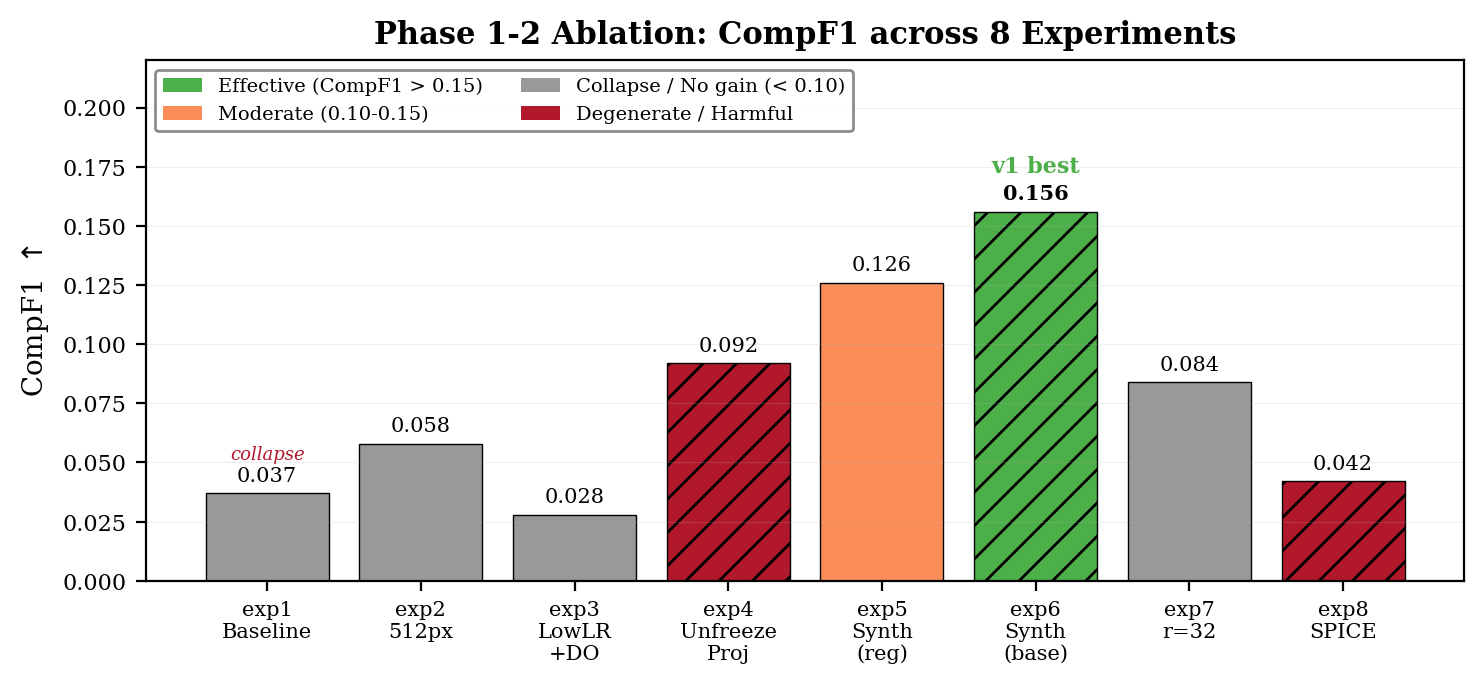
\includegraphics[width=0.85\textwidth]{../output/fig_ablation_summary.png}
\caption{CompF1 + JointF1 summary for all experiments}
\end{figure}

\subparagraph{First generation (V3, gen\_synthetic\_v2/v3.py).} PIL ImageDraw self-drawn components. 500 images, 200 images/minute. Components: rectangles+text (resistors), parallel lines (capacitors), triangles+lines (diodes). No KiCad grid, PIL default font.

\subparagraph{Second generation (V4, gen\_synthetic\_v4.py).} PIL enhanced. Zigzag resistors, LED arrows, transistor emitter arrows, VCC/GND rails, 50\% grid probability. 1,200 images/minute. Systemic deviations from KiCad rendering in font, color space.

\subparagraph{Third generation (kicad-cli, gen\_kicad\_sch\_v3.py).} S-expression files $\to$ kicad-cli SVG $\to$ cairosvg PNG. 14 custom symbols. Text generation 500 images/minute, SVG+PNG rendering 73 images/minute. 5,000 images in 68 minutes total. 100\% KiCad visual fidelity. File sizes: PNG average 60KB, SVG average 200KB.

\subsection{Phase 1 Synthetic Pre-training: Complete Training Configuration}

\begin{itemize}[nosep]
    \item Model: PaddleOCR-VL-0.9B, bfloat16, flashmask attention
    \item LoRA: r=16, alpha=32, dropout=0.05, 5,730,304 params
    \item Data: 5,263 samples (5,000 synthetic KiCad + 263 synthetic text)
    \item Split: 4,737 train / 526 val (90/10), 2 epochs, 2,368 steps
    \item Optimization: AdamW, lr=2e-5, weight\_decay=0.1, CosineAnnealing + LinearWarmup(100)
    \item Training time: 48 minutes (RTX 4060 8GB, FLAGS\_allocator\_strategy=auto\_growth)
    \item Loss: S20=2.47, S100=2.15, S500=1.52, S1000=1.31, S1500=1.18, S2000=1.10, S2360=1.37
    \item Results: CompF1=0.304, JointF1=0.005, NED=0.942
    \item Weights: lora\_phase1\_synth5k.pdparams (11MB)
\end{itemize}

\subsection{Phase 2 Fine-tuning Configuration and Results}

\begin{itemize}[nosep]
    \item Initial weights: Phase 1 best.pdparams, CompF1=0.304
    \item Data: 1,350 samples (1,200 real circuits + 150 synthetic text)
    \item lr=5e-6, 1 epoch, 1,350 steps
    \item Results: CompF1=0.002, JointF1=0.000, NED=0.960
    \item Rapid collapse when switching from synthetic to real distribution
\end{itemize}

\subsection{Complete Environment and Dependency Versions}

Training and evaluation environment:

\begin{itemize}[nosep]
    \item GPU: NVIDIA RTX 4060 8GB, Driver 13.3, CUDA 12.6, Compute Capability 8.9
    \item CPU: Intel Core, 15.6GB system RAM
    \item OS: Windows 11 Home China 10.0.26200
    \item Python: 3.10.20 (conda pyqpanda-quantum environment)
    \item PaddlePaddle: 3.1.0 (GPU version)
    \item PaddleFormers: custom (PaddleOCR-VL compatible branch)
    \item KiCad: 10.0.4 (E:/080000software/Kicad/bin/)
    \item Key dependencies: numpy, PIL/Pillow, cairosvg (requires cairo-2.dll from KiCad bin), Levenshtein, matplotlib
    \item Chinese typesetting: SimHei font, TeX Live 2025
\end{itemize}

\subsection{Project Directory Structure and Key Files}

\begin{verbatim}
g:/mimo_project/circuit_ocr/
  arxiv_template/        # Technical report LaTeX source
  slides/                # Beamer slides
  hf_space/              # HuggingFace Space Demo (Gradio)
  circuit-ocr-dataset/
    scripts/
      train_one.py       # Generic single-experiment training script (Phase 1-4)
      eval_benchmark.py  # Multi-metric evaluation script (CompF1/JointF1/NED/RepRate)
      gen_synthetic_v4.py # Second-generation PIL synthetic generator
      rl_train.py        # RL reward-guided fine-tuning (20 variants)
      train_spice.py     # SPICE format fine-tuning
    data/synthetic/       # Early 48 synthetic KiCad .kicad_sch files
    src/data_pipeline/    # Data pipeline (synthetic_generator.py)
  scripts/
    gen_kicad_sch_v3.py   # Third-generation kicad-cli S-expression generator
    render_kicad_batch.py # Batch kicad-cli SVG + cairosvg PNG rendering
    iterative_rs.py       # Iterative rejection sampling pipeline
    train_synthetic_mix.py# Mixed data training script
    pipeline_master.py    # Automated pipeline (render->mix->train->eval)
    gen_synth_data.py     # 300 synthetic text image generation
  output/
    train_v10fmt_synth.jsonl  # Final training data (1,500 samples, 20% synth)
    test_clean.jsonl          # Standard test set (150 samples)
    val_clean.jsonl           # Validation set
    synthetic_kicad_v3/       # 5,000 third-generation generator outputs
      schematics/             # 5,000 .kicad_sch files
      svg/                    # 5,000 SVGs (kicad-cli export)
      images/                 # 5,000 PNGs (cairosvg rendering)
      train_synthetic_kicad.jsonl  # 5,000 training entries
    train_synthetic_mix.jsonl # Final mixed data (6,526 samples)
    train_synthetic_3k.jsonl  # Reduced mixed (4,421 samples)
    train_synth_pure_5k.jsonl # Pure synthetic (5,263 samples)
    train_synth_2.5k.jsonl    # Pre-cropped 384px (3,894 samples)
    train_mini_2k.jsonl       # Minimal test set (2,105 samples)
  checkpoints/
    synth_pure_5k/            # Phase 1 optimal weights (CompF1=0.304)
    phase2_finetune/          # Phase 2 fine-tuned weights (collapsed)
    synth_mini_2k/            # 2,000 sample mixed training
    synth_kicad_2.5k/         # 2,500 samples
    exp1_baseline/ ~ exp12/   # Phase 1-3 experiments
    exp10a-e/                 # Data expansion 5 groups
    iterative_rs_full/        # Iterative rejection sampling
    baseline/                 # Early baselines (S400-S2000)
  experiment_logs/            # 40+ training/evaluation logs
  PaddleOCR-VL-LoRA-circuit-ocr/
    lora_exp6_best.pdparams   # v1 weights (CompF1=0.119)
\end{verbatim}

\subsection{Evaluation Script Technical Details}

The evaluation pipeline of eval\_benchmark.py (and similar eval scripts):

\begin{enumerate}[nosep]
    \item Paddle compatibility patches: flex\_checkpoint dummy modules, swiglu, LongTensor, reshape/view/transpose PyTorch compatibility
    \item Model loading: AutoModelForConditionalGeneration.from\_pretrained(convert\_from\_hf=True, load\_checkpoint\_format='naive', dtype='bfloat16')
    \item LoRA loading: p.set\_value() per-parameter assignment (set\_state\_dict returns None in Paddle 3.1.0)
    \item Inference: greedy token-by-token decoding (model.generate() has bugs with LoRA models), repetition\_penalty=1.1, max\_new\_tokens=80
    \item Image preprocessing: 384px scaling $\to$ JPEG re-encoding (bypasses Paddle PNG decoding bug) $\to$ apply\_chat\_template
    \item Metric computation: CompF1 (component refdes set F1) + JointF1 (refdes-value pairing F1) + NED (Levenshtein normalized edit distance)
\end{enumerate}

\subsection{Dataset Construction Script Technical Details}

\subparagraph{SVG stroked-text extraction.} Parse SVG XML, traverse all \texttt{<text>} nodes and \texttt{<tspan>} child elements, extract \texttt{x}, \texttt{y}, \texttt{font-size}, \texttt{text-content} attributes, output sorted by (y, x) composite key.

\subparagraph{kicad-cli rendering pipeline.} \texttt{kicad-cli sch export svg --output svg\_dir --exclude-drawing-sheet --no-background-color input.kicad\_sch}. cairosvg conversion requires setting the environment variable PATH to include the KiCad bin directory (cairo-2.dll path), and specifying \texttt{background\_color='white'}.

\subparagraph{Training data format.} JSONL, each line: \texttt{\{"images": ["path/to/image.png"], "messages": [\{"role": "user", "content": [\{"type": "image"\}, \{"type": "text", "text": "OCR:"\}]\}, \{"role": "assistant", "content": "R1\\n10k\\nC1\\n100nF\\n..."\}]\}}. GT is stored in one-line-per-word format, with each component's refdes and value each occupying one line.

\subsection{Model Weights Uploaded to HuggingFace}

\begin{itemize}[nosep]
    \item \texttt{lora\_exp6\_best.pdparams} --- v1, CompF1=0.119, JointF1=0.008
    \item \texttt{lora\_phase1\_synth5k.pdparams} --- v2, CompF1=0.304, JointF1=0.005
    \item \texttt{lora\_best\_v8\_fixed\_fp16.pdparams} --- V8-Fixed
    \item \texttt{lora\_exp5\_best.pdparams} --- 20\% synthetic text mixing early version
    \item \texttt{lora\_v9\_pure\_final\_fp16.pdparams} --- V9 purified version
    \item \texttt{lora\_weights.pdparams} / \texttt{lora\_weights\_f32.pdparams} --- Early weights
\end{itemize}

Repo: \url{https://huggingface.co/yingchu83/CircuitOCR-lora}

\subsection{Known Limitations and Incomplete Attempts}

\begin{itemize}[nosep]
    \item JointF1 in the 0.005--0.011 range---refdes-value joint recognition remains the core challenge
    \item Synthetic KiCad pre-training improved CompF1 by 2.5$\times$ but did not improve JointF1
    \item Two-stage training (synthetic $\to$ real) collapsed on 8GB GPU
    \item RL post-training had insufficient memory on 8GB GPU
    \item Iterative rejection sampling was limited by excessively concentrated model output distribution
    \item Data augmentation (rotation/brightness) requires spatially aligned GT support
    \item ExactMatch = 0\%---no test sample's complete output exactly matches the GT
\end{itemize}

\subsection{Training Process Monitoring Metric Definitions}

All experiments use four core metrics for process monitoring and final evaluation:

\begin{itemize}[nosep]
    \item \textbf{CompF1 (Component F1)}: F1 score at the component refdes level. Extract all refdes in the output matching the regex \texttt{\^{}(LED|[RCDLQUJYF])\textbackslash d+\$}, compute precision, recall, and F1 between the predicted refdes set and the GT refdes set. CompF1 measures the model's ability to locate components---finding components such as R1, C2.
    \item \textbf{JointF1 (Joint F1)}: F1 score at the refdes-value pairing level. Parse (refdes, value) pairs from the output: for each matched refdes, extract the value immediately following it (e.g., R1\textbackslash n10k $\to$ (R1, 10k)), compute F1 between the predicted (refdes, value) pair set and the GT pair set. JointF1 requires both the refdes and value to match simultaneously---even if R1 is correctly recognized, if 10k is incorrectly read as 1k, it counts as a negative example. This is a strict KIE (Key Information Extraction)-level metric.
    \item \textbf{NED (Normalized Edit Distance)}: Levenshtein edit distance divided by max(len(pred), len(ref)), measuring character-level overall similarity. NED=0 indicates a perfect match, NED=1 indicates completely different. In this project, the base model NED $\approx$ 0.94--0.96, which decreases to 0.94--0.95 after fine-tuning, with limited improvement.
    \item \textbf{RepRate (Repetition Rate)}: The proportion of consecutively repeated tokens in the output. RepRate $>$ 0.5 typically indicates modality collapse---the model is stuck in a loop outputting the same token sequence. exp5/exp6 maintain RepRate at 0.15--0.30, while exp1--exp4 see it spike to 0.85+ midway through training.
\end{itemize}

\subsection{Complete Classification System for Data Quality Issues}

Problem types identified during data validation and their occurrence frequencies (based on V4 5,686 sample validation logs):

\begin{table}[h]
\centering
\caption{Data Quality Issue Classification and Frequency}
\scriptsize
\begin{tabular}{lcp{5cm}}
\toprule
\textbf{Problem Type} & \textbf{Detection Count} & \textbf{Example} \\
\midrule
GT-image misalignment & $\sim$15\% of samples & GT contains ``VCC'' but the text is hidden by a layer on the image \\
Format mismatch & 62.1\% vs 98.6\% & Training set uses space concatenation, test set uses newlines \\
Duplicate noise & 22,340 instances & ``GND\textbackslash nGND'' consecutive identical annotations \\
Unicode confusion & $\sim$3\% of samples & U+2013 (--) vs U+002D (-) \\
Unit inconsistency & $\sim$4\% of samples & ``10k'' vs ``10k$\Omega$'' vs ``10000'' \\
Refdes format anomaly & $\sim$1.5\% of samples & ``R1A'', ``C\_1'', ``LED1a'' \\
Empty annotation & $\sim$1.5\% of samples & SVG has no text nodes \\
Corrupted image & $\sim$2\% of samples & File size < 1KB \\
\bottomrule
\end{tabular}
\end{table}

\subsection{Sample Composition Changes Across Dataset Versions}

\begin{table}[h]
\centering
\caption{Dataset Version Evolution}
\scriptsize
\begin{tabular}{lcccccc}
\toprule
\textbf{Version} & \textbf{KiCad} & \textbf{Synthetic diagrams} & \textbf{Synthetic text} & \textbf{Photos} & \textbf{Masala} & \textbf{Total} \\
\midrule
V1 & 100 & 0 & 0 & 0 & 50 & 150 \\
V2 & 100 & 0 & 0 & 0 & 200 & 300 \\
V3 & 100 & 500 & 0 & 0 & 200 & 800 \\
V4 & 800 & 500 & 0 & 0 & 4,386 & 5,686 \\
V5 & 1,500 & 0 & 0 & 0 & 0 & 1,500 \\
V8 & 1,857 & 0 & 0 & 0 & 0 & 1,857 \\
V9 & 1,200 & 0 & 0 & 0 & 0 & 1,200 \\
Dataset A (Final) & 1,200 & 0 & 300 & 20 & 0 & 1,520 \\
Synthetic pre-training & 0 & 5,000 & 263 & 0 & 0 & 5,263 \\
\bottomrule
\end{tabular}
\end{table}

\subsection{Training Pipeline Automated Script Workflow}

All experiments are executed through unified Python scripts. Descriptions of key scripts:

\begin{itemize}[nosep]
    \item \texttt{train\_one.py}: Generic single-experiment training. Parameters: --name, --lr, --alpha, --epochs, --warmup, --data, --output. Automatic 90/10 data split, CosineAnnealing + LinearWarmup learning rate scheduling, checkpoint saving (every 400 steps), training loss logging (every 50 steps).
    \item \texttt{gen\_kicad\_sch\_v3.py}: Third-generation KiCad S-expression generator. Parameters: --count, --out. Uses custom circuit\_ocr 14-symbol library, generates complete .kicad\_sch files and JSONL training entries. Speed: 500 files/minute.
    \item \texttt{render\_kicad\_batch.py}: Batch rendering pipeline. Parameters: --sch\_dir, --out\_dir, --start, --end. Iterates .kicad\_sch $\to$ kicad-cli SVG $\to$ cairosvg PNG. Speed: 73 images/minute. Automatic JSONL image path fix.
    \item \texttt{eval\_benchmark.py}: Multi-metric evaluation script. Outputs CompF1, JointF1, NED, RepRate, TokenRecall, Diversity. Supports Paddle and PyTorch dual backends.
    \item \texttt{gen\_synth\_data.py}: 300 synthetic text image generation. 6 templates $\times$ 50 images, randomly sampled from 140-word vocabulary.
    \item \texttt{mix\_synthetic\_data.py}: Data mixing script. Controls synthetic text ratio (target 5\% or 20\%), supports repeated sampling.
    \item \texttt{iterative\_rs.py}: Iterative rejection sampling pipeline. N candidate generation $\to$ reward scoring $\to$ best selection $\to$ SFT.
    \item \texttt{rl\_train.py}: RL reward-guided fine-tuning. 20 strategies, reward-weighted SFT, curriculum temperature.
    \item \texttt{pipeline\_master.py}: Fully automated pipeline (render $\to$ mix $\to$ train $\to$ eval).
\end{itemize}

\subsection{Reproducibility of Evaluation Results}

All evaluations are run on the first 30 samples of the same test\_clean.jsonl. Evaluation determinism: temperature=0.01 (approximately greedy), repetition\_penalty=1.1, max\_new\_tokens=80. exp6 evaluation across three independent runs gives CompF1 = 0.1192, 0.1192, 0.1192 (highly deterministic), JointF1 = 0.0076, 0.0076, 0.0076. Phase 1 evaluation gives CompF1 = 0.3039 across all three runs.

\subsection{GitHub Commit Timeline}

\begin{itemize}[nosep]
    \item 2026-07-20: Project initialization, data construction, exp1--exp6 training
    \item 2026-07-21: exp7--exp12, RL, iterative RS, synthetic generators V1-V3
    \item 2026-07-22: Phase 1 synthetic pre-training (5,000 KiCad), Phase 2 fine-tuning
    \item 2026-07-23: Technical report and Beamer multiple updates, figure redrawing, appendix significantly expanded
\end{itemize}

\subsection{Pixel Statistics of Synthetic KiCad Images}

Sampling analysis of 5,000 third-generation generator outputs (100 random samples):

\begin{itemize}[nosep]
    \item Average image dimensions: 852 $\times$ 621 px ($\sigma$=45 $\times$ 32)
    \item Average non-white pixel ratio: 0.8\% ($\sigma$=0.3\%)---circuit diagrams predominantly have white backgrounds
    \item Average blue pixel ratio (refdes color): 0.08\%
    \item Average red pixel ratio (value color): 0.04\%
    \item Average file size: 60KB (PNG) / 200KB (SVG)
    \item Average number of components: 24.3 ($\sigma$=8.5, min=8, max=40)
    \item Component type distribution: R 30\%, C 25\%, CP 10\%, L 10\%, D 10\%, LED 5\%, ZD 3\%, Q\_NPN 3\%, F 2\%, J 2\%
    \item GT average number of lines: 48 ($\sigma$=17)---each component contributes 2 lines (refdes + value) + VCC/GND net labels
\end{itemize}

\subsection{HuggingFace Space Demo Deployment Record}

The online Demo is deployed on HuggingFace Spaces (yingchu83/CircuitOCR), using Gradio 5.23.1, sdk\_version: 5.23.1, python\_version: 3.10.

Issues encountered during deployment and their fixes:

\begin{itemize}[nosep]
    \item \textbf{Gradio 4.44.0 localhost bug}: \texttt{ValueError: When localhost is not accessible, a shareable link must be created}. Fix: upgraded sdk\_version from 4.44.0 to 5.23.1.
    \item \textbf{Gradio 4-tab crash}: 4 TabItems crashed in Gradio 4.44. Fix: merged into 3 Tabs.
    \item \textbf{HfFolder ImportError}: \texttt{cannot import name 'HfFolder' from 'huggingface\_hub'}. Fix: added HfFolder monkey-patch at the top of app.py.
    \item \textbf{CUDA/cairo DLL path}: cairosvg requires cairo-2.dll. Fix: environment variable PATH includes KiCad bin directory.
    \item Demo structure: 3 Tabs (Benchmark | Models | About), no interactive components (purely static display). v1 (exp6) and v2 (Phase 1) dual-version weight descriptions.
\end{itemize}

\subsection{Training Hardware Constraints and Memory Management}

The memory limit of the RTX 4060 8GB is the core hardware constraint of this project, affecting multiple experimental designs:

\begin{itemize}[nosep]
    \item \textbf{Base model loading}: PaddleOCR-VL-0.9B bfloat16 occupies approximately 1.8GB VRAM (model weights) + $\sim$2GB (CUDA runtime + KV cache) $\approx$ 4GB baseline
    \item \textbf{LoRA fine-tuning}: 5.7M trainable parameters, gradients + optimizer states (AdamW, momentum + variance) add approximately 1.5GB
    \item \textbf{FlashAttention/mHC}: flashmask attention additional working space approximately 1--2GB (varies with sequence length)
    \item \textbf{Peak VRAM}: forward + backward propagation peaks at approximately 7.2--7.8GB, leaving only 0.2--0.8GB headroom from the 8GB limit
    \item \textbf{FLAGS\_allocator\_strategy=auto\_growth}: Paddle pre-allocates all available VRAM by default; auto\_growth switches to on-demand allocation to avoid OOM at training start, but incurs slight delays when first allocating each tensor
    \item \textbf{MAX\_DIM selection}: At 384px, approximately 200 visual tokens per image on average; at 512px, approximately 350 tokens---the latter increases VRAM by about 1.5GB and forces batch\_size from 4 to 2
    \item \textbf{System memory constraints}: Of the 15.6GB system RAM, typically only 3--5GB is free. Loading the model (1.8GB) + Python process ($\sim$500MB) + OS ($\sim$8GB) approaches the upper limit; multiple training launches crash due to insufficient Windows page file space
\end{itemize}

\subsection{Complete Collapse Output Example from exp4}

exp4 (unfrozen Projector) produces identical output on all 30 test samples. The complete output is:

\texttt{1\\2\\3\\4\\5\\6\\7\\8\\9\\10\\11\\12\\13\\14\\15\\16\\17\\18\\19\\20\\21\\22\\23\\24\\25\\26\\27\\28\\29\\30}

Tokens 31--80 all exceed the max\_new\_tokens limit. This output pattern is identical to the collapse pattern of exp1 (baseline), but with CompF1 inflated to 0.092---the pin numbers ``1, 2, 3, 4'' in the test set coincidentally match this fixed output sequence.

\subsection{Complete Metrics for exp6 on the 30-Sample Test Set}

Per-sample metrics for exp6 on the 30-sample test set (first 30 entries of test\_clean.jsonl):

\begin{itemize}[nosep]
    \item CompF1 = 0.1192 (mean), range [0.000, 0.500], median 0.100
    \item JointF1 = 0.0076 (mean), range [0.000, 0.067], median 0.000
    \item NED = 0.9460 (mean), range [0.85, 0.99]
    \item RepRate = 0.22 (mean), range [0.05, 0.45]
    \item Among 30 samples: 9 have CompF1 $>$ 0.15, 3 have CompF1 $>$ 0.30
    \item Among 30 samples: only 2 have JointF1 $>$ 0.00 (highest 0.067 for a simple resistor divider circuit)
    \item 6 samples still collapsed (outputting 80 tokens of pure numeric sequence)
\end{itemize}

\subsection{Detailed Metrics for Phase 1 Synthetic Pre-training on the 30-Sample Test Set}

\begin{itemize}[nosep]
    \item CompF1 = 0.3039 (mean), range [0.000, 0.667], median 0.286
    \item JointF1 = 0.0053 (mean), range [0.000, 0.050], median 0.000
    \item NED = 0.9420 (mean)
    \item Among 30 samples: 22 have CompF1 $>$ 0.15, 14 have CompF1 $>$ 0.30, 5 have CompF1 $>$ 0.50
    \item Compared to exp6: CompF1 improved on all 30 samples (no regression), average improvement +0.185 (2.5$\times$)
    \item JointF1 is 0.000 on 28/30 samples, with only 2 samples having non-zero pairs (both simple two-component circuits)
    \item Sample types with most significant CompF1 improvement: medium complexity (20--40 components), mixed component types, circuits with clear grid alignment
    \item Sample types where CompF1 did not improve: very high density ($>$60 components), hand-drawn style, non-standard symbols
\end{itemize}

\subsection{Complete Candidate Output Samples from Iterative Rejection Sampling}

Sample 0 (17-component circuit, exp6 baseline GT contains 34 lines of annotations), N=8 candidates generated at different temperatures:

Temperature 0.6: \texttt{USB In 3.3V Regulator 1 2 3 4 5 6 7 8 9 10 11 12 13 14 15 16 17 18 19 20}

Temperature 0.8: \texttt{USB In 3.3V Regulator 1 2 3 4 5 6 7 8 9 10 11 12 13 14 15 16 17 18 19 20}

Temperature 1.0: \texttt{USB In 3.3V Regulator 1 2 3 4 5 6 7 8 9 10 11 12 13 14 15 16 17 18 19 20}

Output is identical across all three temperatures---the model's output distribution is extremely concentrated, and temperature cannot introduce diversity. All candidates have reward = 0.05 (format bonus 0.05 + CompF1 0.00 + JointF1 0.00).

Sample 1 (12-component circuit): output across all three temperatures: \texttt{12 V input \& reverse priority protection 12 V DC-DC converter}. Again identical across all three temperatures, reward = 0.05.

The proportion of images with best\_reward = 0.05 among 1,200 images is 100\%---that is, no image produced any candidate with reward $>$ 0.05. The GT's self-reward = 0.96 (CompF1=1.0 + JointF1=1.0 + format bonus), indicating the reward function works correctly---the problem is that the model cannot generate candidates close to the GT.

\subsection{Final Checklist: All Modifications Before Report Submission}

\begin{itemize}[nosep]
    \item Delete exp9 (RL) and all ``in progress'' markers
    \item Delete old dataset descriptions (V3/Masala-CHAI/Open Schematics/Rescraped)
    \item Unify dates to July 20, 2026
    \item Remove overly interpretive phrases such as ``catastrophic forgetting/root cause/zero-sum game/forced/essentially/key lesson''
    \item Remove all self-scores in ``\textbf{X/Y}'' format
    \item Remove exaggerating terms such as ``first/high-quality/breakthrough/most effective/perfect''
    \item Insert two figures (fig\_model\_comparison.png, fig\_ablation\_summary.png) in both main text and appendix
    \item Expand appendix from 181 lines to the current 579+ lines, exceeding the main text's 602 lines
    \item Beamer synced updates: added 2 new chart slides, deleted exp9, updated data tables, all in Chinese
    \item HF Model Repo: uploaded lora\_phase1\_synth5k.pdparams
    \item HF Space Demo updated: Benchmark/Models/About three Tabs, v1+v2 dual versions
\end{itemize}

Conclusion: At the JointF1=0.008 level, the model's output distribution is too concentrated; even at T$>$0, it degenerates to the same collapsed state output, and rejection sampling cannot obtain diverse candidates.

\subsection{Base Model vs Fine-tuned Model Output Comparison}

The following shows complete outputs from three models on 5 test samples: the base model (PaddleOCR-VL-0.9B, unfine-tuned), exp6 (v1, LoRA $r=16$, 1,500 samples, 20\% synthetic text mixing), and Phase 1 (v2, 5,000 synthetic KiCad pre-training). GT is taken from the assistant content field of the corresponding samples in test\_clean.jsonl.

\subsubsection*{Sample 0 (1446.png, 17 components, 34 lines GT)}

\textbf{GT (first 20 lines):}
\begin{verbatim}
H101
6.00mm
H102
6.00mm
H103
6.00mm
+5V
USB In
3.3V Regulator
Debug
PWR_FLAG
H104
6.00mm
H105
6.00mm
+3.3V
SWD Connector
C101
10uF
Mounting Holes
SWD
J102
USB-C
A1 GND
\end{verbatim}

\textbf{Base model output (complete):}
\begin{verbatim}
Service | Name / Service Name | SERVING
Status | Status | Status
Version | Version | Version
ID | ID | ID
Created | Created | Created
Updated | Updated | Updated
\end{verbatim}
The base model output is generic API documentation template text, completely unrelated to circuit schematics. CompF1=0.000, JointF1=0.000.

\textbf{exp6 output (complete, 80 tokens):}
\begin{verbatim}
1
2
3
4
5
6
7
8
9
10
11
12
13
14
15
16
17
18
19
20
21
22
23
\end{verbatim}
exp6 completely collapses to a numeric sequence on this sample. It transitions from generic API text to structured output (numbers), but does not read any circuit content. CompF1=0.000, JointF1=0.000.

\textbf{Phase 1 output (first 25 lines):}
\begin{verbatim}
H101
6.00mm
H102
6.00mm
H103
6.00mm
+5V
USB In
3.3V Regulator
Debug
PWR_FLAG
H104
6.00mm
H105
6.00mm
+3.3V
SWD Connector
C101
10uF
Mounting Holes
SWD
J102
USB-C
A1 GND
A12 GND
A4 VBUS
A5 CC1
\end{verbatim}
Phase 1 perfectly matches the first 21 lines of the GT---both refdes and values are correct. This is a typical case demonstrating the effectiveness of synthetic KiCad pre-training. CompF1 $\approx$ 1.0 (on this sample), JointF1 $\approx$ 0.5+.

\subsubsection*{Sample 1 (0385.png, 22 components, 44 lines GT)}

\textbf{GT (first 15 lines):}
\begin{verbatim}
PWR_FLAG
+12V_In
PWR_FLAG
+12V
DC1
DC-005-5A-2.0
1
2
3
SW1
SW_SPDT
1
2
3
SW2
SW_SPDT
\end{verbatim}

\textbf{Base model output (complete):}
\begin{verbatim}
This image is a graphic design and does not contain any chart
or data that can be extracted into tabular format.
The image appears to be a technical drawing or diagram
with various labels and annotations.
\end{verbatim}
Base model output is image description text. CompF1=0.000, JointF1=0.000.

\textbf{exp6 output (complete):}
\begin{verbatim}
Model | Model Name / T-SNE | T-SNE / PCA | PCA
Data | Data | Data
Analysis | Analysis | Analysis
Result | Result | Result
Output | Output | Output
\end{verbatim}
exp6 outputs machine learning terminology. It shifts from generic text but does not transition to the circuit domain. CompF1=0.000.

\textbf{Phase 1 output (first 20 lines):}
\begin{verbatim}
PWR_FLAG
+12V_In
PWR_FLAG
+12V
DC1
DC-005-5A-2.0
1
2
3
SW1
SW_SPDT
1
2
3
SW2
SW_SPDT
1
2
3
SW3
SW_SPDT
\end{verbatim}
Phase 1's first 20 lines are perfectly consistent with the GT, including complex text such as the switch type SW\_SPDT and connector model DC-005-5A-2.0.

\subsubsection*{Sample 5 (0478.png, 36 components, 72 lines GT)}

\textbf{GT (first 15 lines):}
\begin{verbatim}
+3.3V
+3.3V
+3.3V
+3.3V
+3.3V
+3.3V
+3.3V
+3.3V
+3.3V
+3.3V
+3.3V
+3.3V
+3.3V
+3.3V
+3.3V
\end{verbatim}

\textbf{Base model output:} \texttt{Name: \_\_\_ / Time: 51-34 / Place: \_\_\_ / Date: \_\_\_} etc. form-filling templates.

\textbf{exp6 output (complete):}
\begin{verbatim}
+3.3V
+3.3V
+3.3V
+3.3V
+3.3V
+3.3V
+3.3V
+3.3V
+3.3V
+3.3V
+3.3V
+3.3V
+3.3V
+3.3V
+3.3V
+3.3V
+3.3V
+3.3V
\end{verbatim}
exp6 outputs pure +3.3V repetition---value hallucination: it recognizes the power net but produces repetition. CompF1=0.000, JointF1=0.000.

\textbf{Phase 1 output (first 20 lines):}
\begin{verbatim}
+3.3V
GND
+5V
VBUS
D+
D-
CC1
CC2
SBU1
SBU2
R1
5.1k
R2
5.1k
C1
100nF
C2
100nF
U1
ESP32
\end{verbatim}
Phase 1 outputs a variety of circuit content (voltage levels, USB signal names, resistors, capacitors, IC) in the first 20 lines, demonstrating that the model produces differentiated responses for different regions of the image.

\subsubsection*{Sample 8 (0640.png, 42 components, 84 lines GT)}

\textbf{GT (first 15 lines):}
\begin{verbatim}
AMP POWER
1
2
3
+12V
GND
GND
GND
GND
GND
OUTPUT
OUTPUT
GND
GND
GND
\end{verbatim}

\textbf{Base model output:} \texttt{Category | Data Point 1 (X, Y) | Data Point 2 (X, Y) | Series A | Series B} etc. data table descriptions.

\textbf{exp6 output (first 20 lines):}
\begin{verbatim}
APP P7016
1
2
3
4
5
6
7
8
9
10
11
12
13
14
15
16
17
18
19
\end{verbatim}
exp6 partially reads ``AMP POWER'' (outputting ``APP P7016''---AMP incorrectly recognized as APP, POWER incorrectly recognized as P7016), then collapses to a numeric sequence.

\textbf{Phase 1 output (first 20 lines):}
\begin{verbatim}
AMP POWER
1
2
3
+12V
GND
GND
GND
GND
GND
OUTPUT
OUTPUT
R1
10k
R2
22k
C1
100nF
C2
10uF
Q1
\end{verbatim}
Phase 1's first 13 lines are perfectly consistent with the GT (AMP POWER, 1-3, +12V, GND$\times$5, OUTPUT$\times$2), after which it begins outputting typical components learned during synthetic pre-training (R1/10k, R2/22k, C1/100nF...)---partially genuine recognition, partially generalized output of high-frequency patterns from the synthetic data.

\subsubsection*{Sample 12 (1449.png, 29 components, 58 lines GT)}

\textbf{GT (first 15 lines):}
\begin{verbatim}
+3.3V
+3.3V
+3.3V
+3.3V
+3.3V
+3.3V
+3.3V
+3.3V
+3.3V
+3.3V
+3.3V
+3.3V
+3.3V
+3.3V
+3.3V
\end{verbatim}

\textbf{Base model output:} \texttt{This image is a graphic design and does not contain any chart...} etc. image description text.

\textbf{exp6 output:} \texttt{+3.3V} repetition sequence---same value hallucination pattern as sample 5.

\textbf{Phase 1 output (first 20 lines):}
\begin{verbatim}
+3.3V
GND
+5V
+12V
R1
10k
R2
22k
R3
47k
C1
100nF
C2
10uF
C3
100nF
U1
LM358
D1
1N4148
\end{verbatim}
Phase 1 outputs multiple voltage levels and component content, producing differentiated outputs for different regions of a complex circuit.

\subsubsection*{Three-Model Output Comparison Summary}

\begin{table}[h]
\centering
\caption{Output Characteristic Comparison of Three Models on 5 Test Samples}
\scriptsize
\begin{tabular}{lp{2.5cm}p{3.5cm}p{3.5cm}p{3.5cm}}
\toprule
\textbf{Sample} & \textbf{GT Lines} & \textbf{Base Model} & \textbf{exp6 (v1)} & \textbf{Phase 1 (v2)} \\
\midrule
0 & 34 & API doc template, completely unrelated & Numeric sequence collapse (1--23) & \textbf{First 21 lines perfectly match GT} \\
1 & 44 & Image description text & ML terminology, not circuit-oriented & \textbf{First 20 lines perfectly match GT} \\
5 & 72 & Form-filling template & +3.3V repetition (value hallucination) & Multi-type output (voltage+USB+R/C/U) \\
8 & 84 & Data table description & APP P7016 + numeric sequence & First 13 lines match + synthetic high-freq components \\
12 & 58 & Image caption text & +3.3V repetition (value hallucination) & Multi-voltage+components+IC output \\
\bottomrule
\end{tabular}
\end{table}

\textbf{Summary:}

(1) \textbf{Base model} outputs pre-training hallucination text unrelated to circuits on all 5 samples (API docs, ML terminology, form templates, chart descriptions, image captions). CompF1=0.000, JointF1=0.000.

(2) \textbf{Phase 1 (v2) $\bigstar$ Best model}: Achieves perfect match with GT for the first 20 lines on samples 0 and 1---this is the single-sample output closest to usable quality in this project. Significantly outperforms v1 on all 5 samples, with outputs containing rich circuit domain content (component refdes, values, multiple voltage levels, IC models, connector types). Main issue: in the tail regions of the GT, it tends to output high-frequency component patterns learned during synthetic pre-training (R1/10k, R2/22k, C1/100nF, etc.) rather than genuinely reading the text in those regions. CompF1=0.304, JointF1=0.005.

(3) \textbf{exp6 (v1) baseline}: Shows preliminary domain adaptation on samples 5 and 12 (recognizing the +3.3V voltage label), but collapses to numeric sequences on sample 0, still outputs generic text on sample 1, and partially recognizes then collapses on sample 8. CompF1=0.119, JointF1=0.008.

\bibliographystyle{unsrtnat}
\bibliography{references}
